Four-top-quark final states are characterised by a high multiplicity of reconstructed objects and a rich internal structure. 
Each top quark decays predominantly via $t \to Wb$, leading to final states containing multiple energetic jets, several $b$-tagged jets, isolated leptons, and significant missing transverse momentum. 
Signal events therefore populate regions of phase space with large jet multiplicity and substantial hadronic activity.

The dominant background, primarily $t\bar{t}+\mathrm{jets}$, shares many of these features. 
Additional jets arising from initial- and final-state radiation can mimic the high jet multiplicities characteristic of signal events. 
While simple observables such as $H_T$, jet multiplicity, and $b$-tag multiplicity provide partial separation, their individual discriminating power is limited. 
The essential difference between signal and background lies not only in global event activity but also in the correlated structure of reconstructed objects.

In such high-dimensional final states, angular separations, invariant mass combinations, and decay-topology patterns carry significant information. 
Capturing these correlations in a systematic way motivates the use of multivariate techniques capable of learning non-trivial relationships among reconstructed objects.

In this analysis, a mass-parameterised Graph Neural Network (GNN) classifier is employed to discriminate the heavy Higgs boson signal from the dominant Standard Model background. 
GNNs operate on graph-structured representations of events, naturally accommodating variable object multiplicities and explicitly encoding relationships between reconstructed objects. 
By incorporating the heavy Higgs boson mass as an input feature, a single classifier can be trained across multiple signal mass hypotheses, enabling smooth interpolation between mass points and maximising the use of available signal statistics.

\subsection{Mass-parameterised Graph Neural Network Classifier}

The detailed construction and training strategy of the mass-parameterised GNN classifier are presented in this section. 
The network operates on graph representations of reconstructed events and explicitly includes the Higgs boson mass hypothesis as an additional input feature.

The training is performed in signal-enriched regions defined by high jet and $b$-tag multiplicities. 
For the single-lepton (1L) channel, events are required to contain at least nine jets and at least three $b$-tagged jets, while for the opposite-sign dilepton (2LOS) channel the requirement is at least seven jets and at least three $b$-tagged jets. 
Signal samples corresponding to Higgs boson masses between $400$ and $1000~\mathrm{GeV}$ in steps of $100~\mathrm{GeV}$ are used for training.

A mass-parameterised training strategy is adopted by providing the Higgs-boson mass hypothesis, $m_H$, as an additional input. 
For signal events, $m_H$ is set to the true benchmark mass of the simulated sample, while for background events a pseudo-mass is assigned by sampling uniformly from the same discrete set of benchmark masses. 
The classifier therefore learns a decision function $s(x,m_H)$ that depends explicitly on the mass hypothesis. 
This enables a single network to interpolate across mass points and share statistical information between different signal benchmarks, avoiding the need for separate classifiers.

To ensure stable and unbiased training, event weights are rescaled such that each signal mass hypothesis contributes equally to the loss function and signal and background yields are balanced within each mass slice. 
The loss is computed using binary cross entropy and is evaluated per event, weighted by the absolute event weight before averaging over each batch.

Events are encoded as graphs $G=(\mathbf{u}, V, E)$, where $\mathbf{u}$ denotes global event features, $V$ is the set of nodes corresponding to reconstructed objects, and $E$ represents pairwise relationships between objects. 
The graph is constructed as a fully connected directed graph without self-connections.

Each reconstructed jet, electron, muon, and the missing transverse momentum ($E_{\mathrm{T}}^{\mathrm{miss}}$) is represented as a node. 
The node feature vector contains:
\begin{itemize}
    \item Transverse momentum $p_{\mathrm{T}}$,
    \item Pseudorapidity $\eta$ (set to zero for $E_{\mathrm{T}}^{\mathrm{miss}}$),
    \item Energy $E$,
    \item Pseudo-continuous DL1r $b$-tagging score (zero for non-jet objects),
    \item Object-type encoding.
\end{itemize}
The azimuthal angle $\phi$ is not included as an explicit node feature; instead, relative geometric information is captured through edge features, ensuring invariance under global rotations in the transverse plane.

Edges are defined between all ordered pairs of nodes and encode geometric relationships in the $(\eta,\phi)$ plane. 
The edge feature vector consists of:
\begin{itemize}
    \item $\Delta\phi$,
    \item $\Delta\eta$,
    \item $\Delta R$.
\end{itemize}

In addition to node and edge information, a set of global features $\mathbf{u}$ is included to provide high-level event descriptors such as $H_T$, jet multiplicity, invariant mass combinations, and substructure-related observables. 
These global features complement the relational information encoded in the graph while avoiding redundancy with explicit node inputs.

The network follows the standard message-passing paradigm in which edge, node, and global representations are iteratively updated through trainable neural networks. 
No architectural modifications beyond this generic framework are introduced. 
The implementation uses the \texttt{PyTorch Geometric} library and consists of several message-passing layers followed by a fully connected layer producing a binary classification score $y \in [0,1]$.

The main hyperparameters of the network are:
\begin{itemize}
    \item Number of message-passing layers: 3 (1L) and 2 (2LOS),
    \item Hidden dimension: 32 units,
    \item Dropout probability: 0.10 (1L) and 0.25 (2LOS),
    \item Optimiser: Adam with learning rate $10^{-3}$,
    \item Loss function: Binary cross entropy.
\end{itemize}

To control potential overfitting, a two-fold cross-training procedure is employed. 
Events are split according to their event number into even and odd subsets. 
Two independent models are trained, each evaluated on the complementary subset, and the final discriminant score used in the analysis corresponds to the prediction obtained from the model that did not see the event during training.

During statistical interpretation, a separate profile likelihood fit is performed for each target mass point $m_H^\ast$. 
For each hypothesis, classifier outputs are evaluated using the corresponding mass input for both signal and background samples, thereby reproducing the behaviour of mass-specific classifiers within a unified parameterised framework.

\subsection{Validation and Performance}

The robustness of the mass-parameterised GNN classifier is assessed through overtraining checks, comparisons of score distributions, and dedicated studies of the mass-parameterisation behaviour.

The difference between training and testing AUC values is used to quantify overfitting. 
In the 1L channel this difference remains below $1\%$ for all mass points, while in the 2LOS channel it is at the level of approximately $2\%$, indicating stable training.

Representative classifier score distributions for several benchmark mass points are shown in Figure~\ref{fig:1l-gnn-scores} for the 1L channel and in Figure~\ref{fig:2los-gnn-scores} for the 2LOS channel. 
A clear separation between signal and background is observed in both channels. 
The agreement between training and testing distributions further confirms the stability of the model. 
As expected, the separation improves for higher Higgs-boson masses, reflecting the increased kinematic differences between signal and background at larger mass scales.

\begin{figure}[htbp]
  \centering
  \begin{subfigure}[t]{0.32\textwidth}
    \centering
    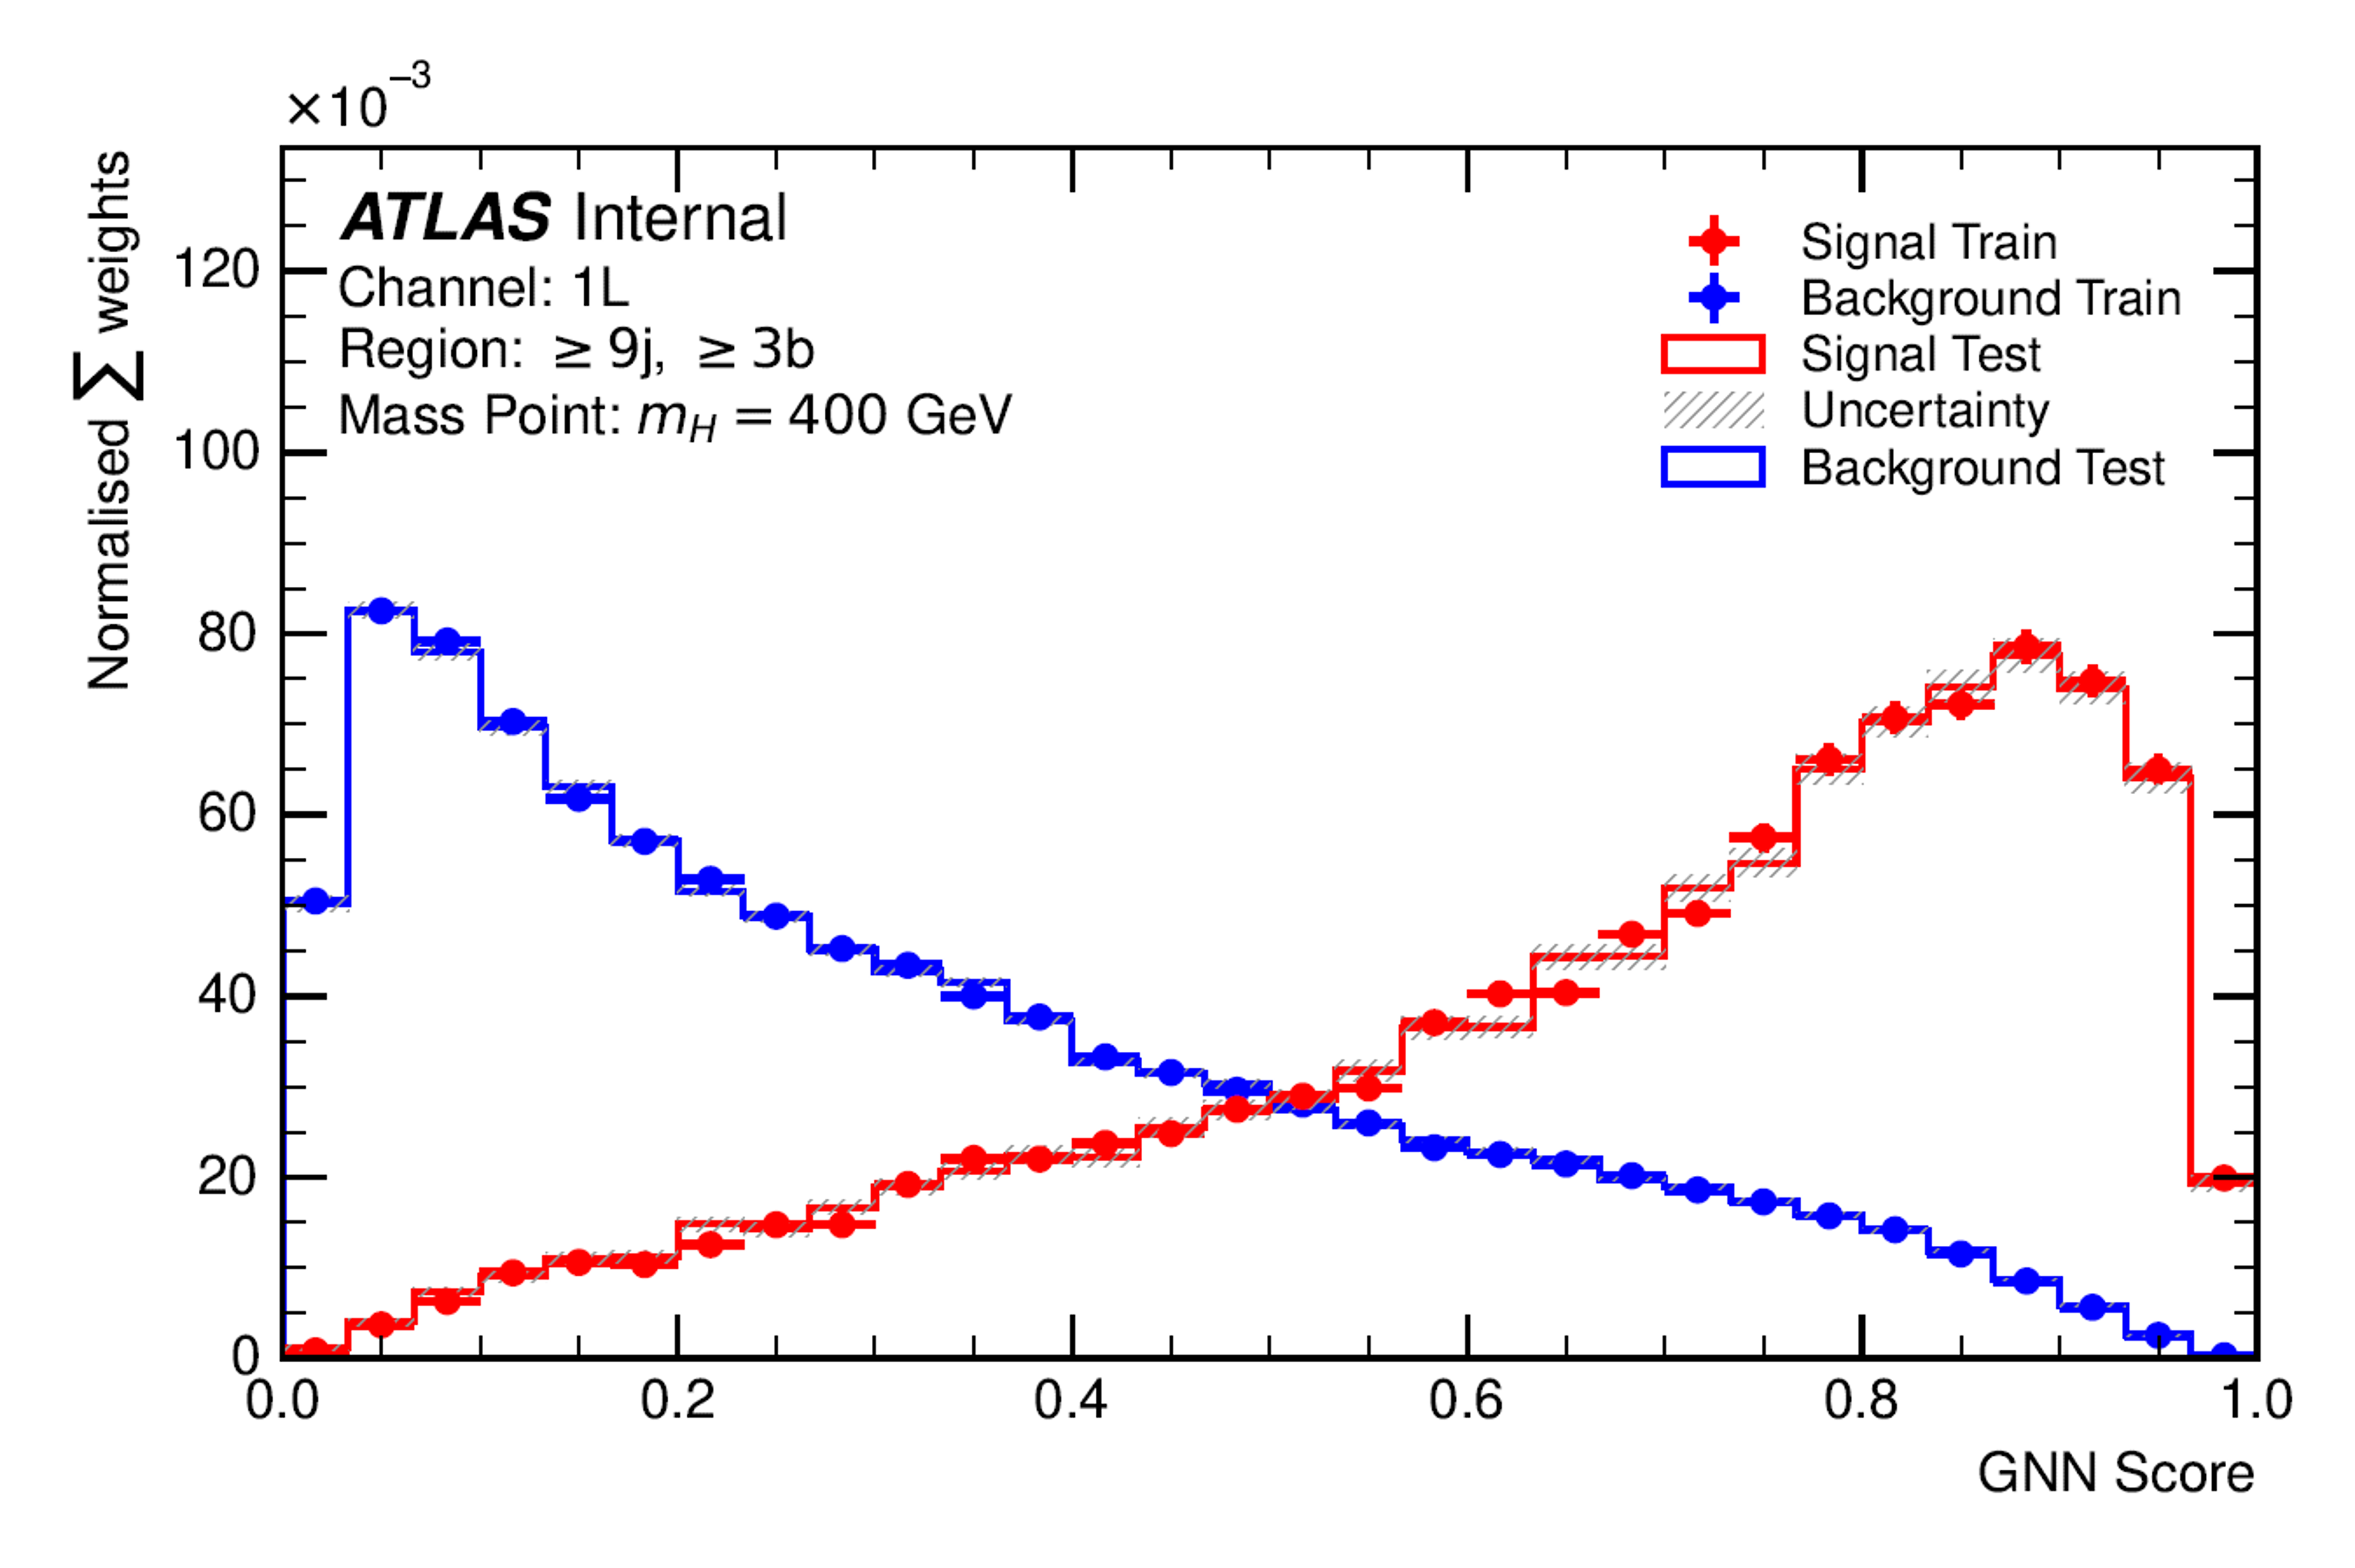
\includegraphics[width=\textwidth]{figures/gnn/Plots_1L/400/GNN_Score_Plot_400GeV_Inclusive.png}
    \caption{$m_H=400~\mathrm{GeV}$}
  \end{subfigure}\hfill
  \begin{subfigure}[t]{0.32\textwidth}
    \centering
    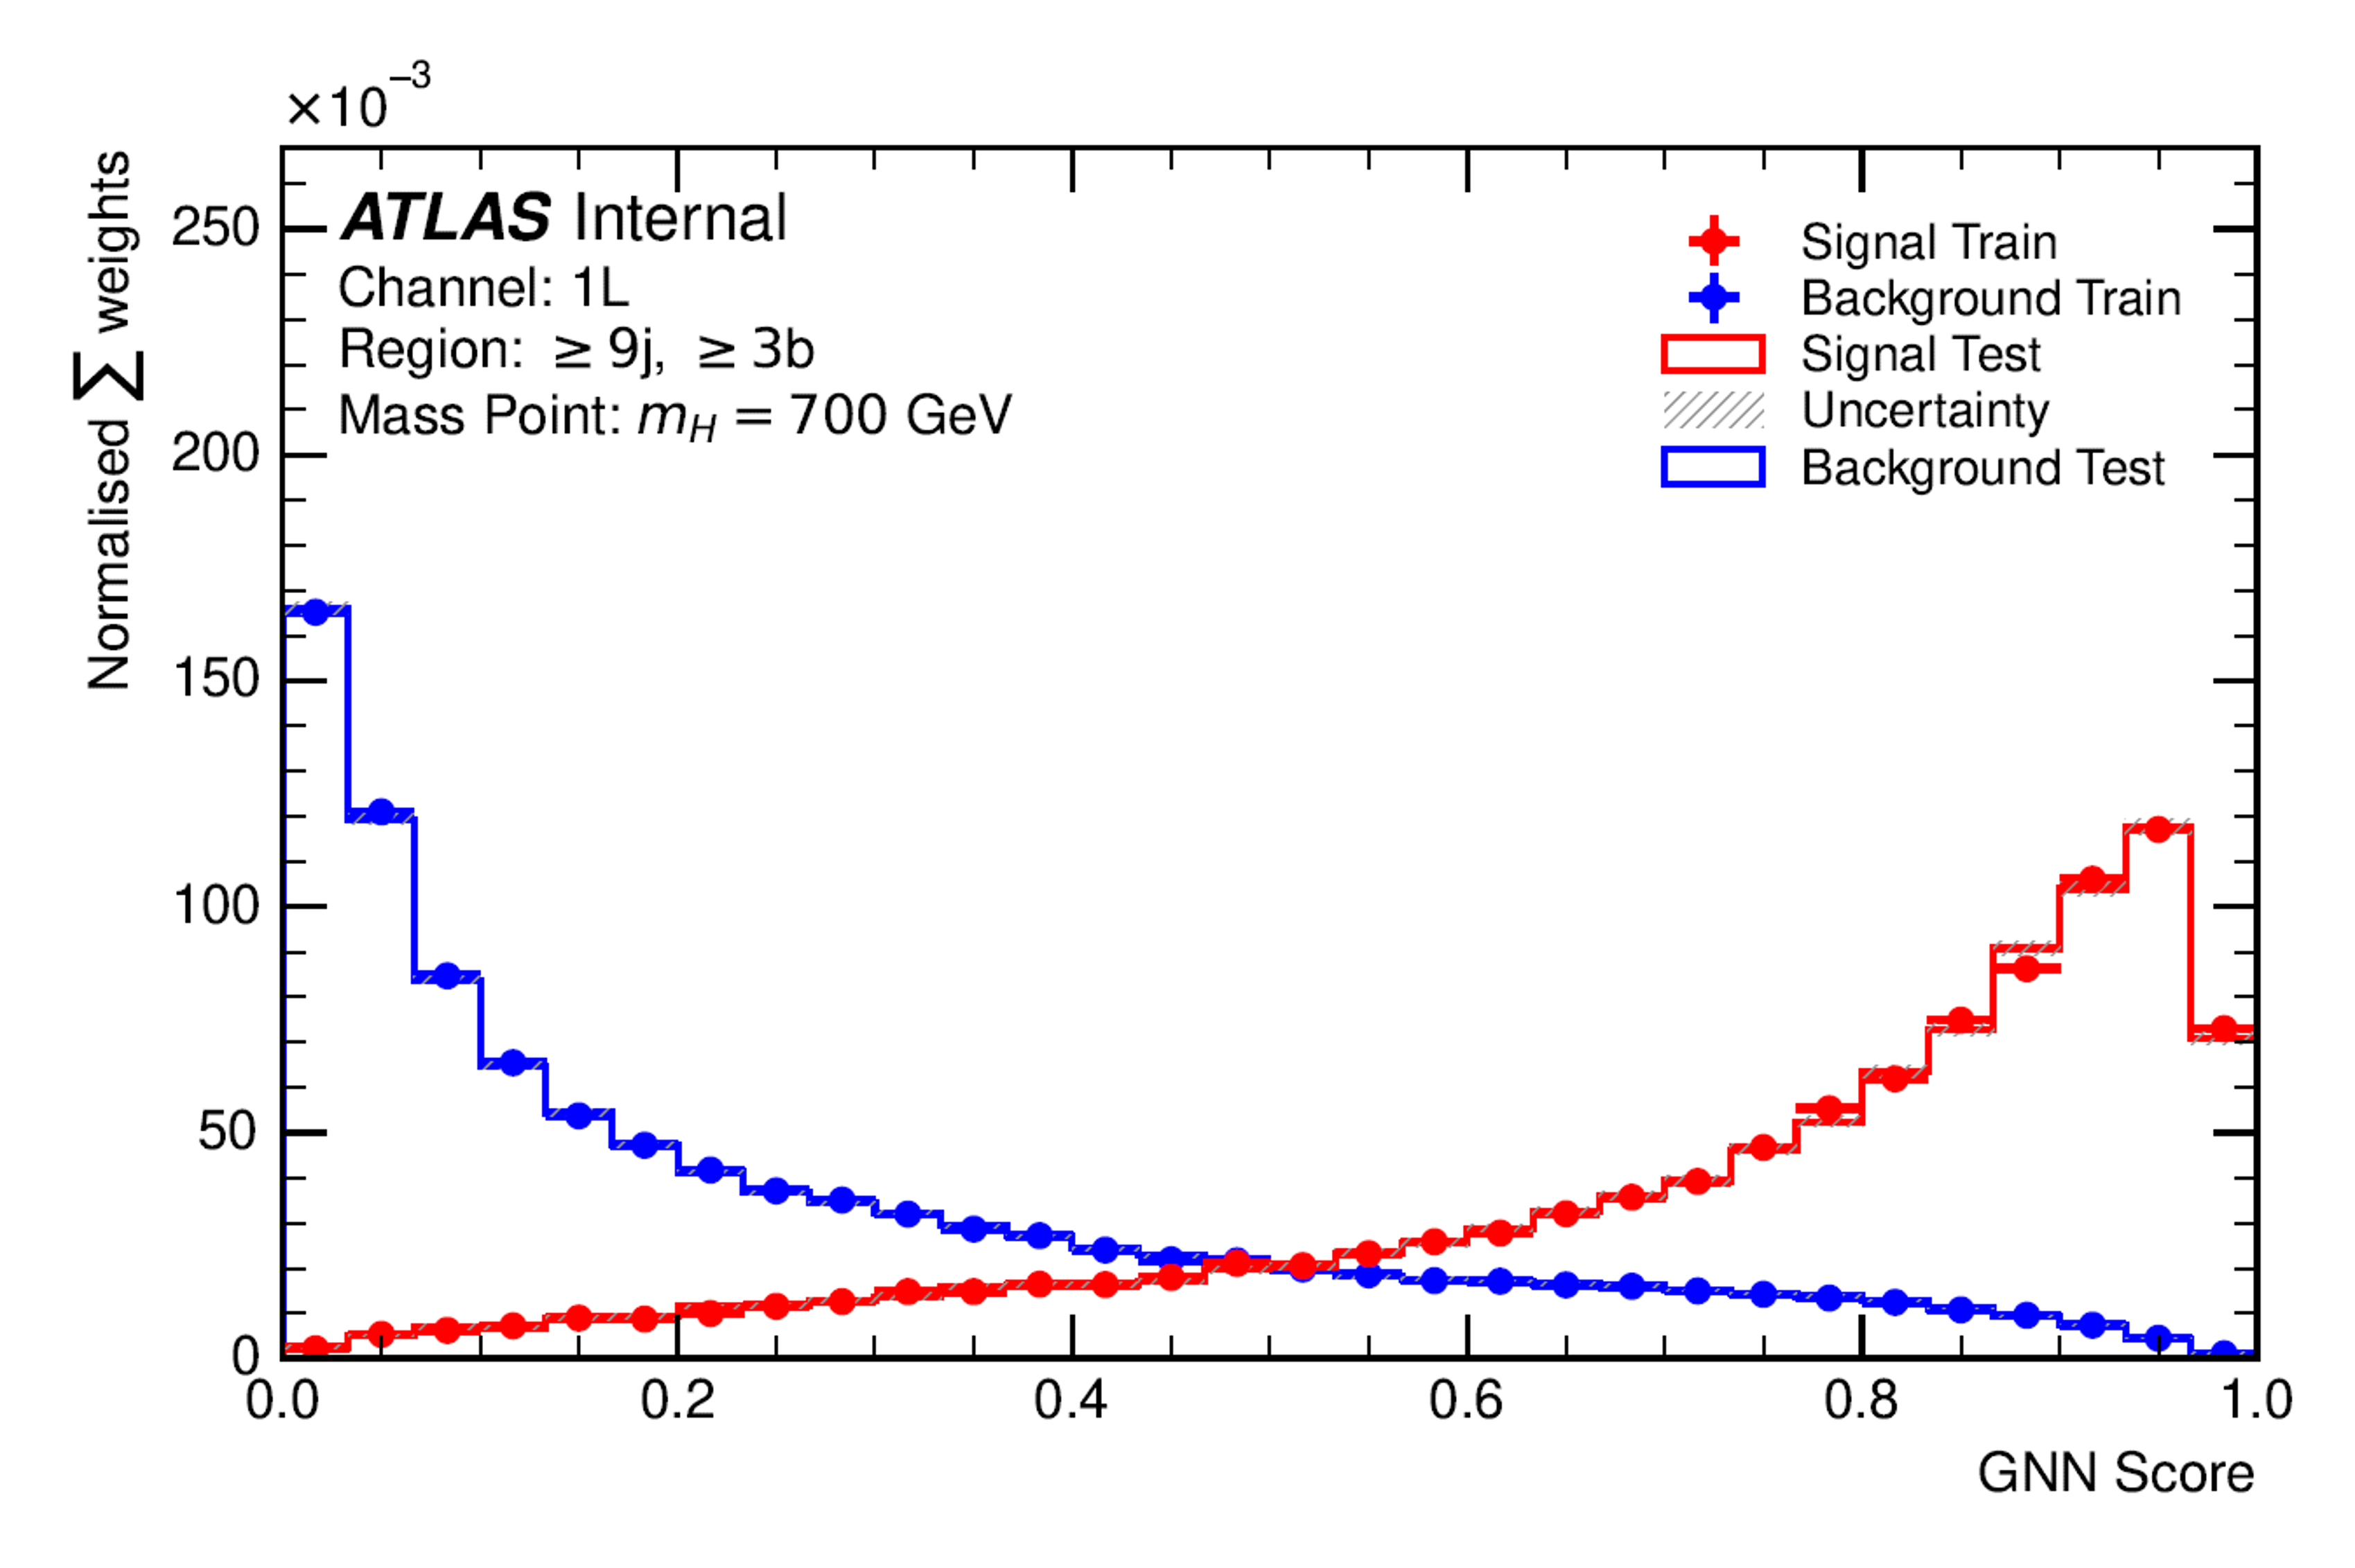
\includegraphics[width=\textwidth]{figures/gnn/Plots_1L/700/GNN_Score_Plot_700GeV_Inclusive.png}
    \caption{$m_H=700~\mathrm{GeV}$}
  \end{subfigure}\hfill
  \begin{subfigure}[t]{0.32\textwidth}
    \centering
    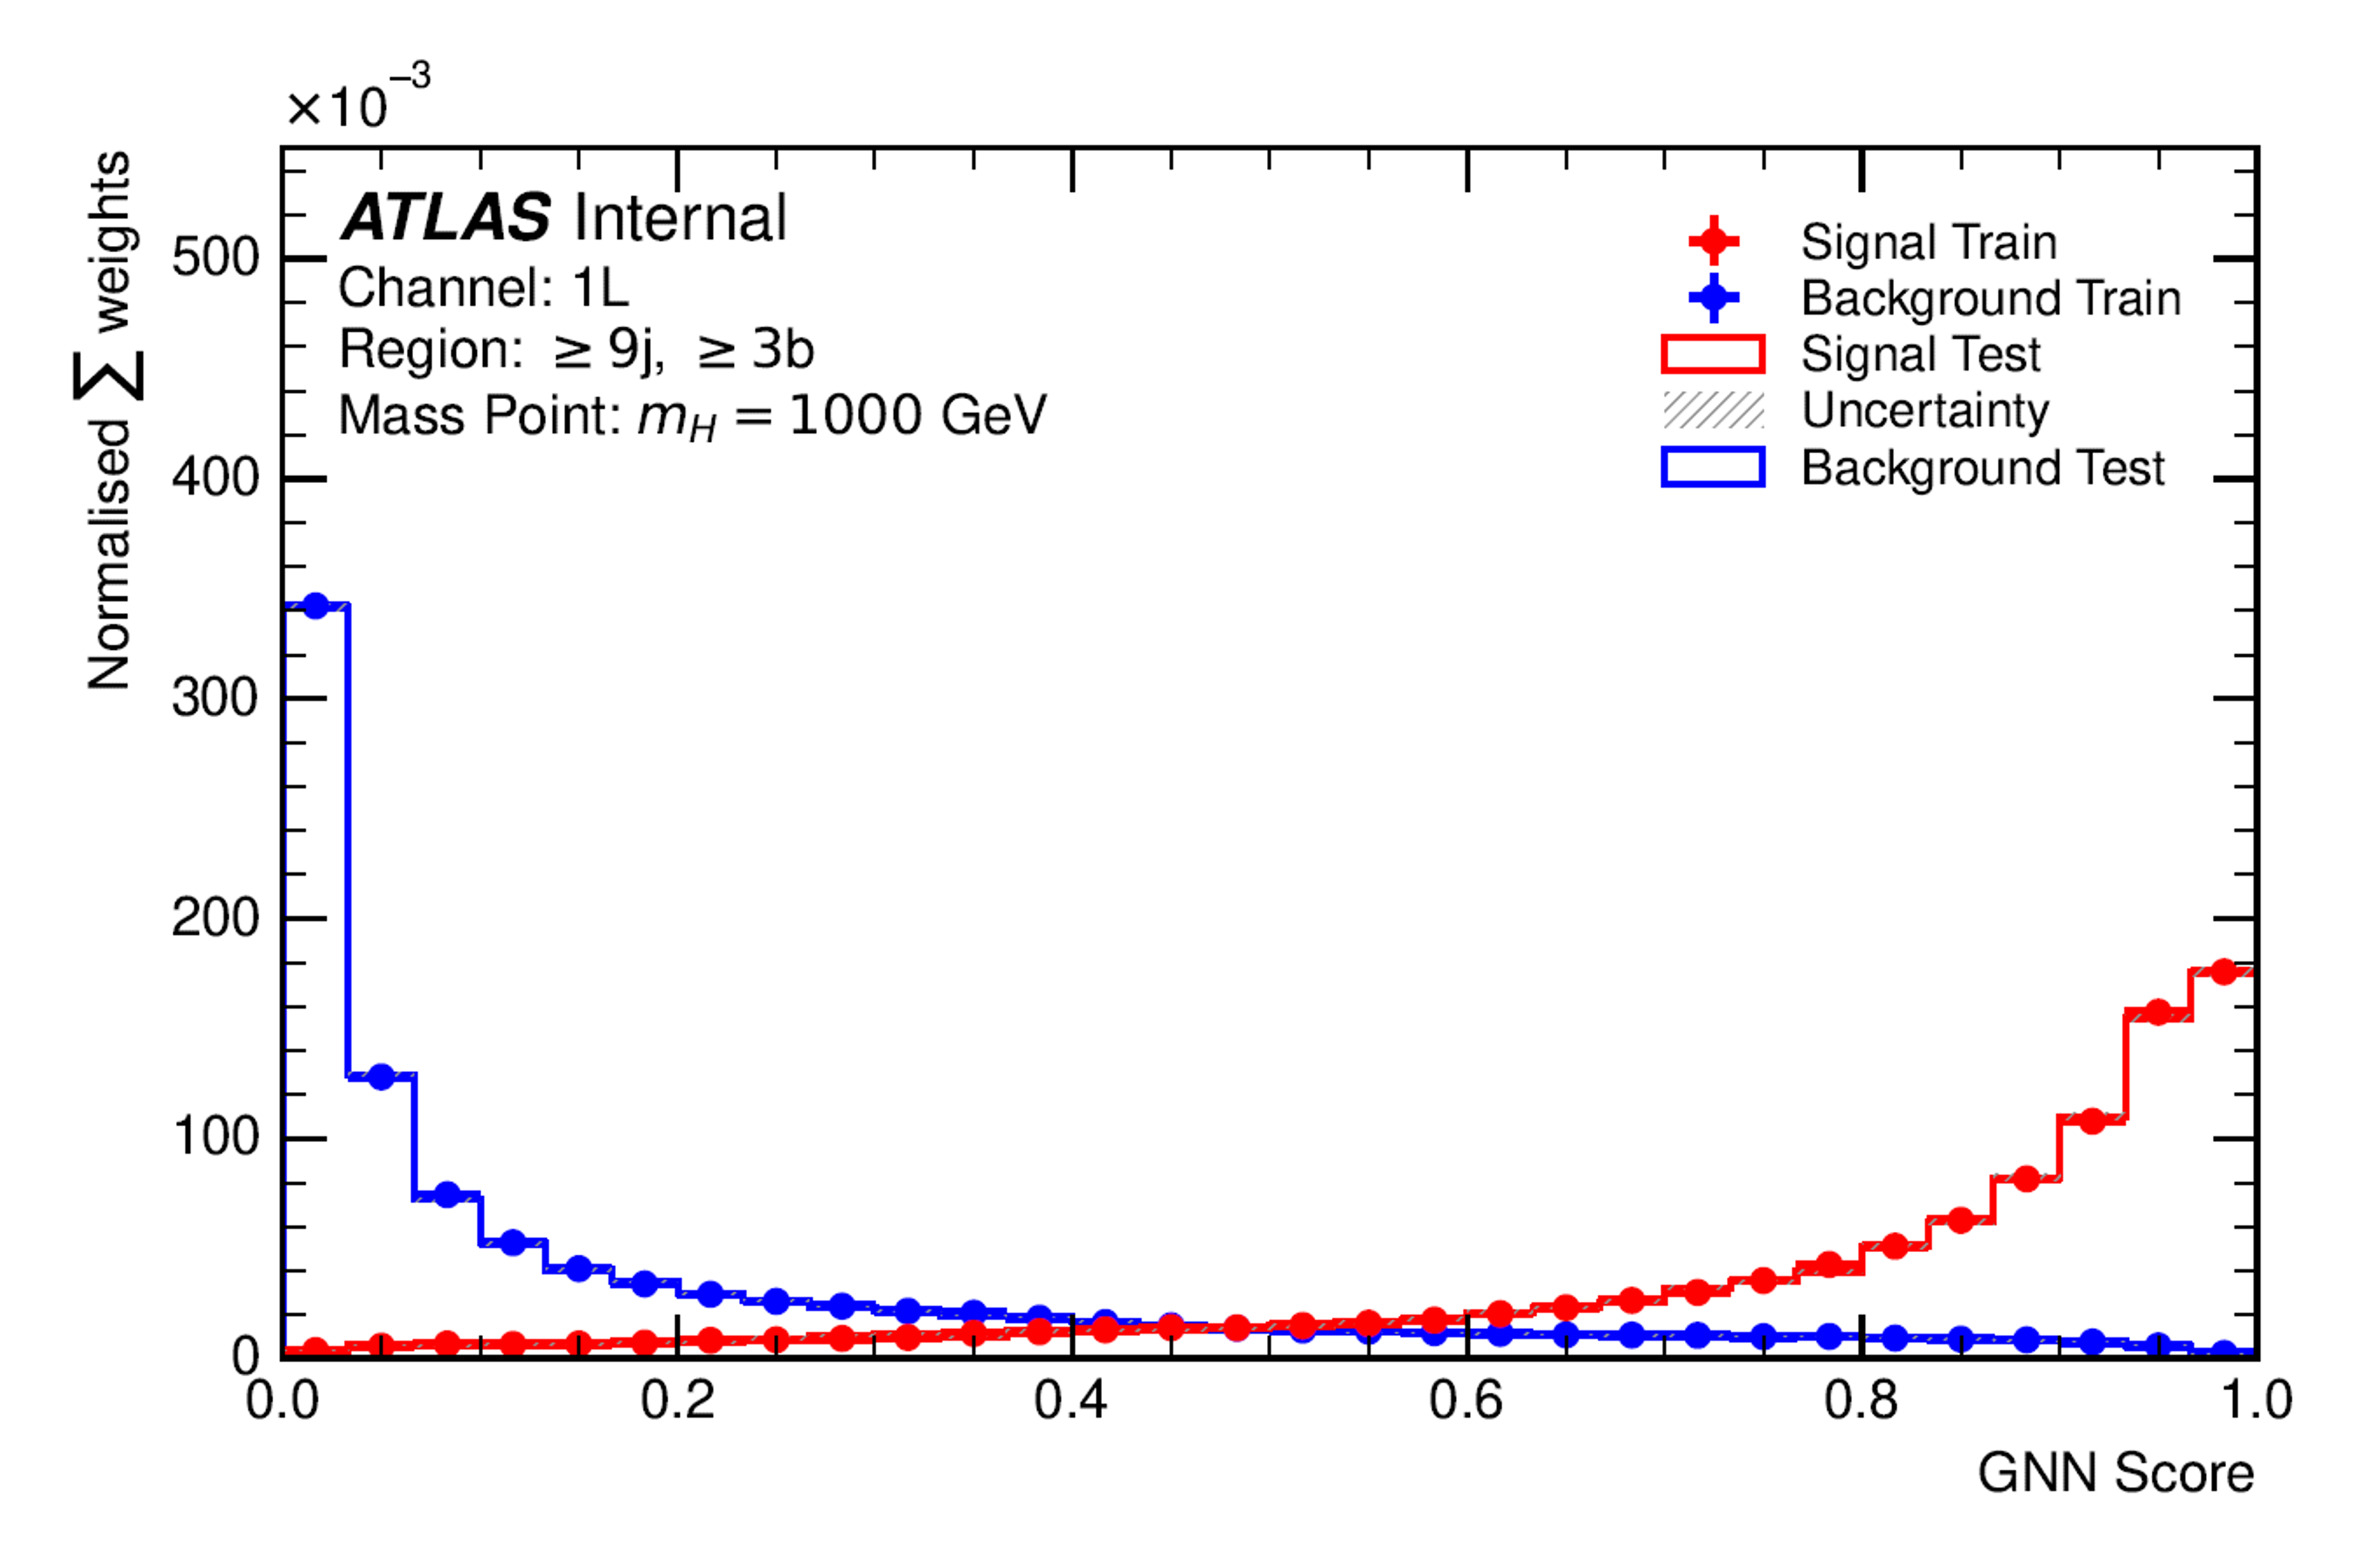
\includegraphics[width=\textwidth]{figures/gnn/Plots_1L/1000/GNN_Score_Plot_1000GeV_Inclusive.png}
    \caption{$m_H=1000~\mathrm{GeV}$}
  \end{subfigure}
  \caption{GNN score distributions in the 1L channel for representative Higgs-boson mass hypotheses in the inclusive training region.}
  \label{fig:1l-gnn-scores}
\end{figure}

\begin{figure}[htbp]
  \centering
  \begin{subfigure}[t]{0.32\textwidth}
    \centering
    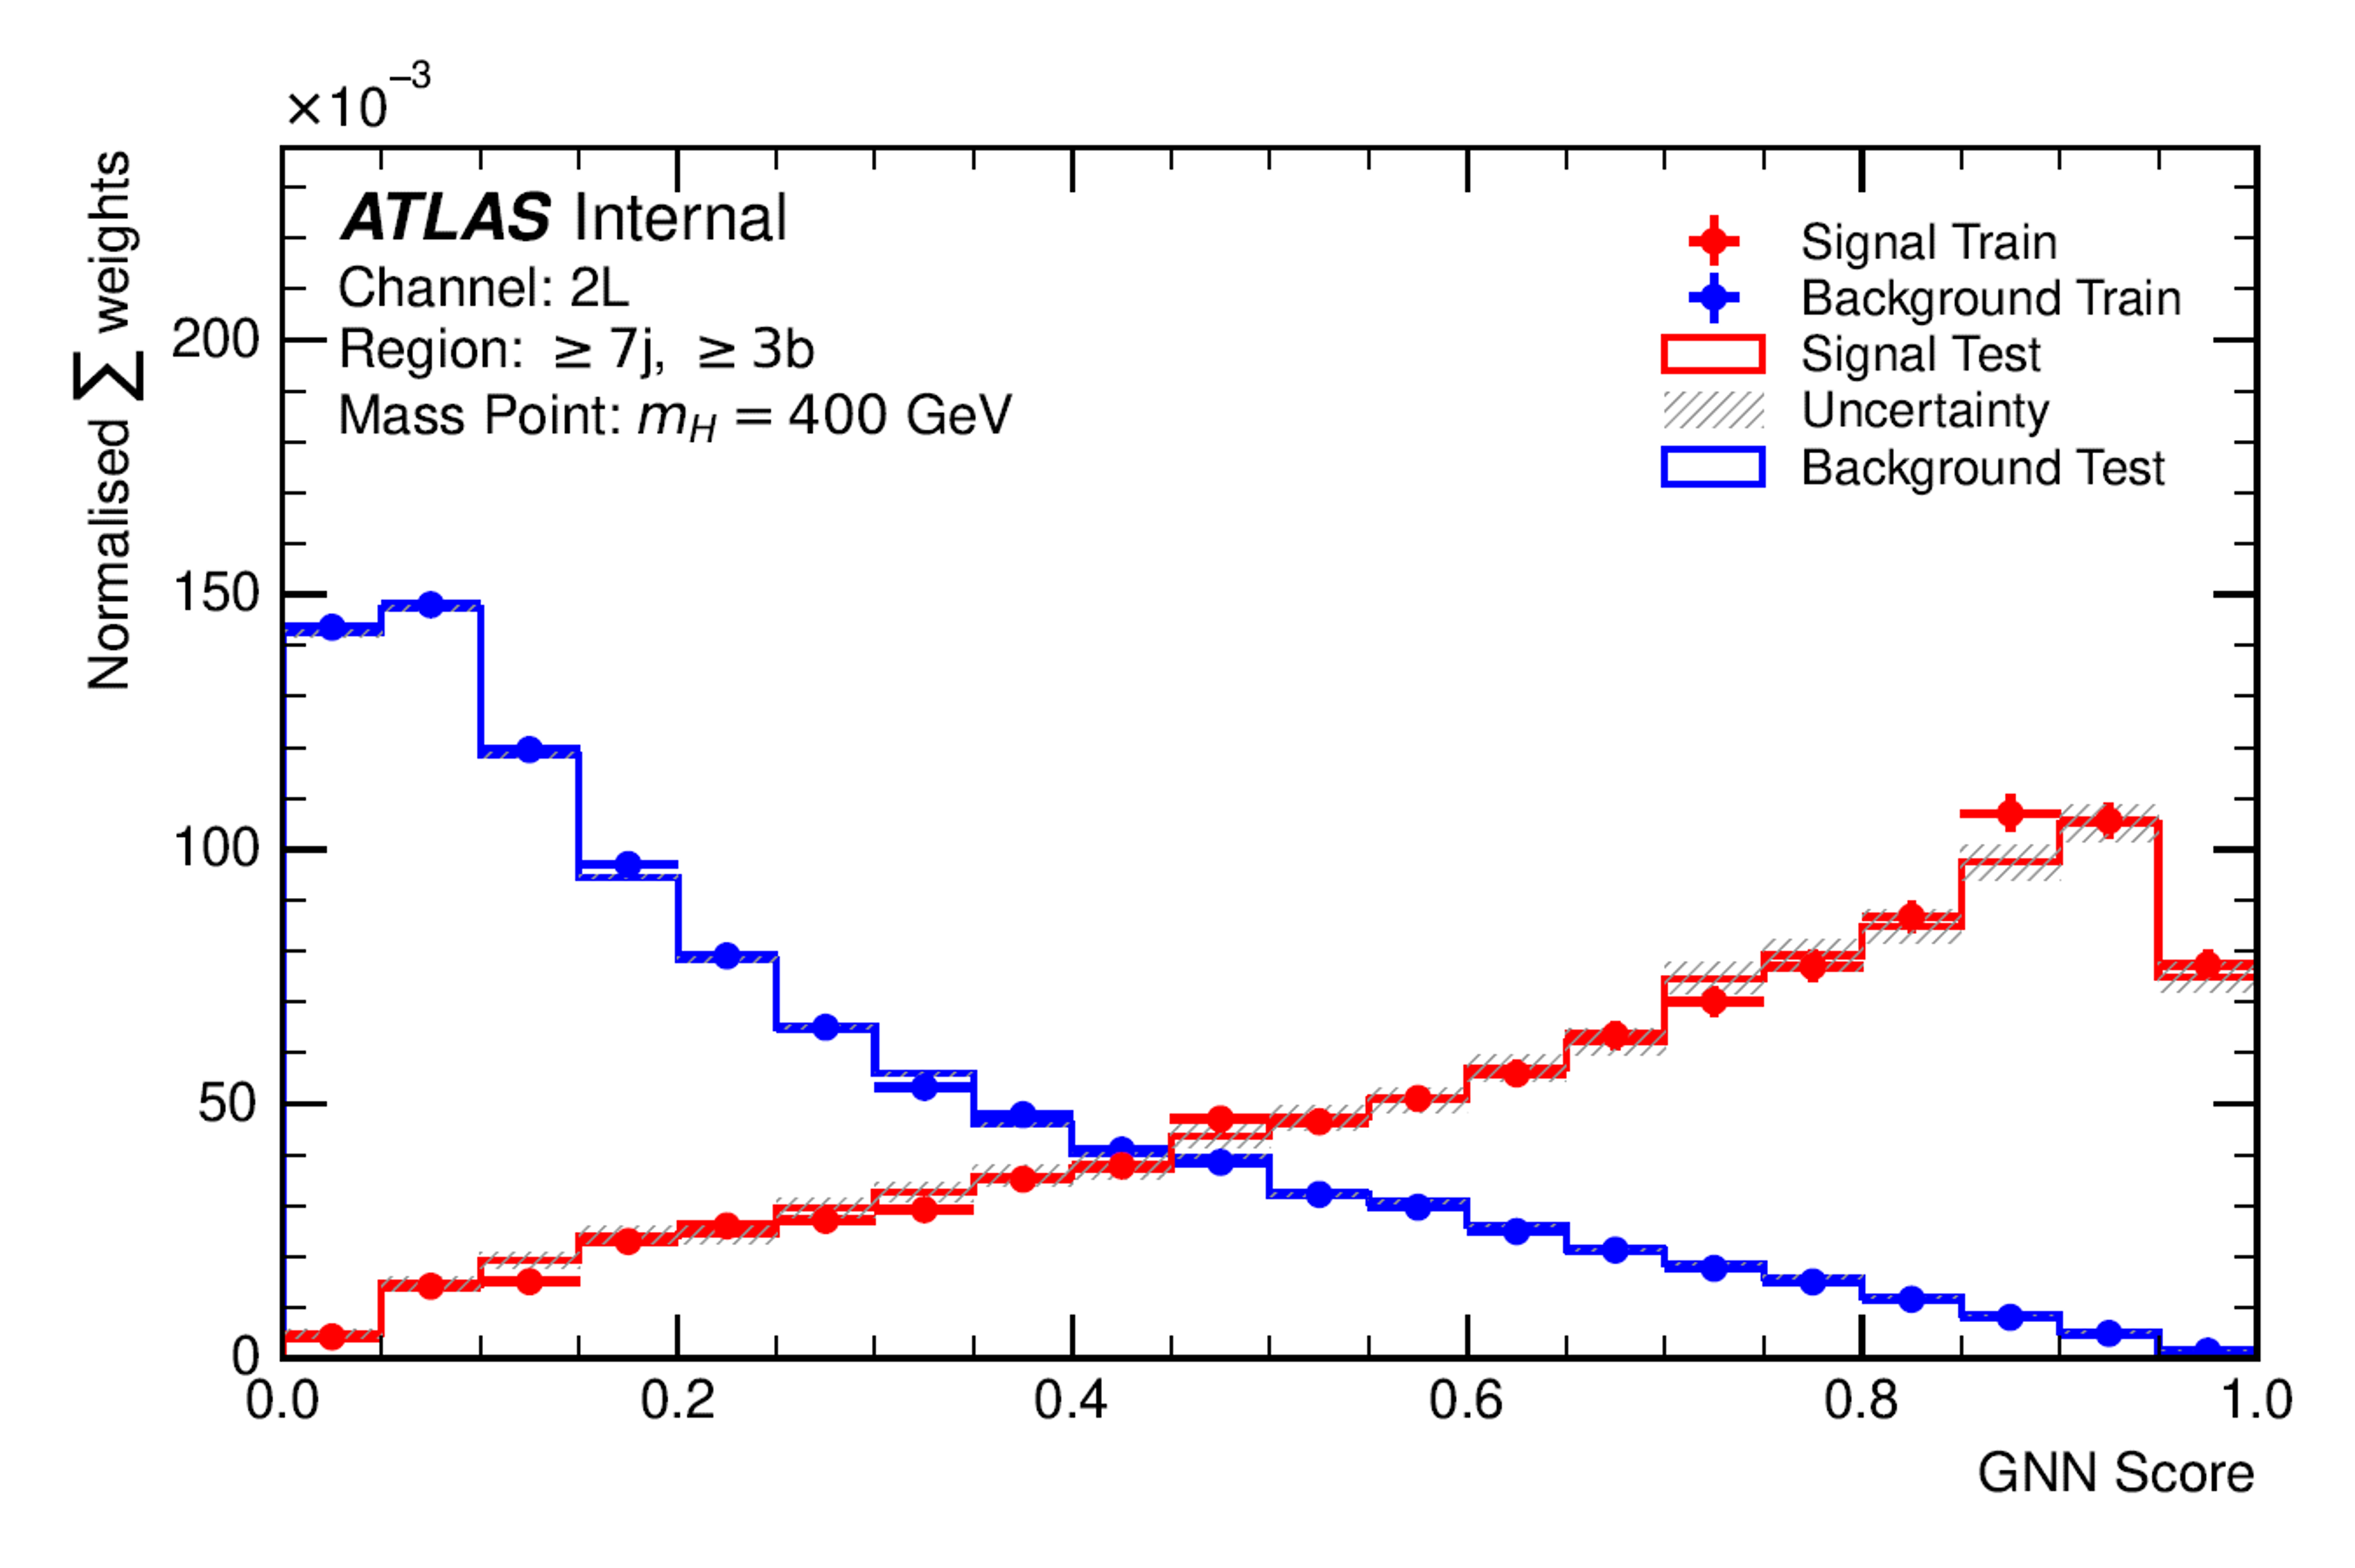
\includegraphics[width=\textwidth]{figures/gnn/Plots_2LOS/400/GNN_Score_Plot_400GeV_Inclusive.png}
    \caption{$m_H=400~\mathrm{GeV}$}
  \end{subfigure}\hfill
  \begin{subfigure}[t]{0.32\textwidth}
    \centering
    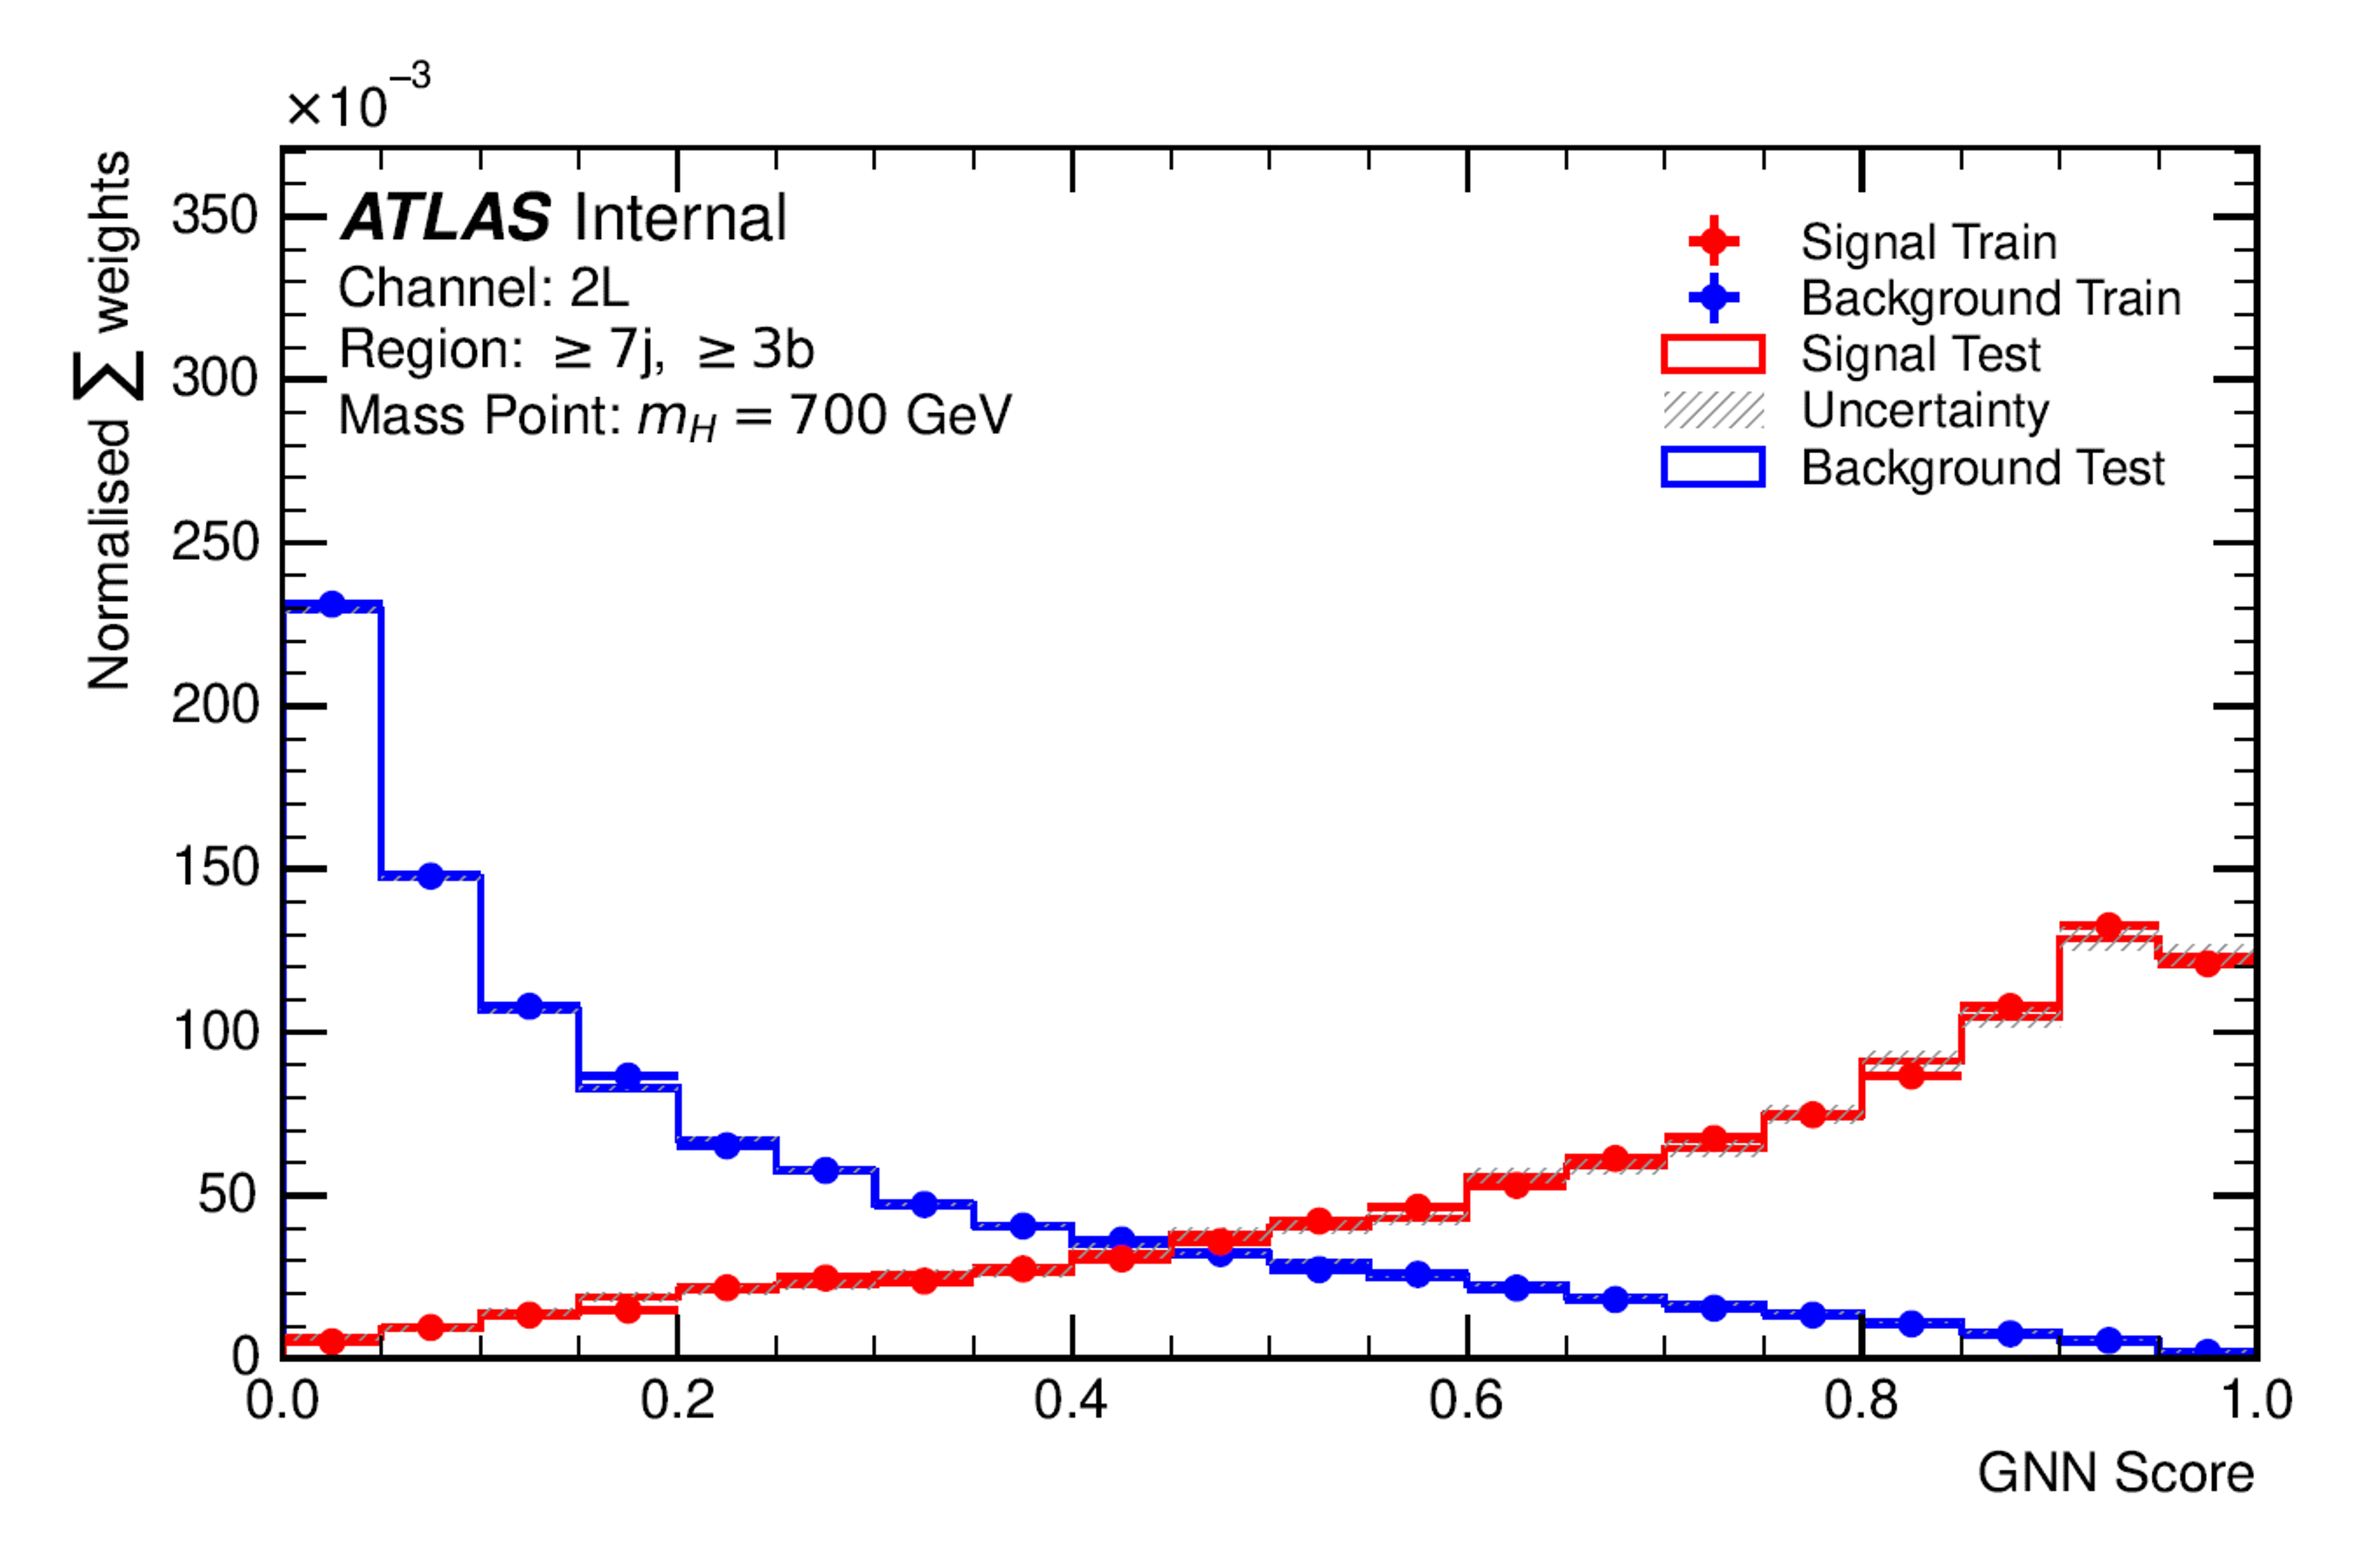
\includegraphics[width=\textwidth]{figures/gnn/Plots_2LOS/700/GNN_Score_Plot_700GeV_Inclusive.png}
    \caption{$m_H=700~\mathrm{GeV}$}
  \end{subfigure}\hfill
  \begin{subfigure}[t]{0.32\textwidth}
    \centering
    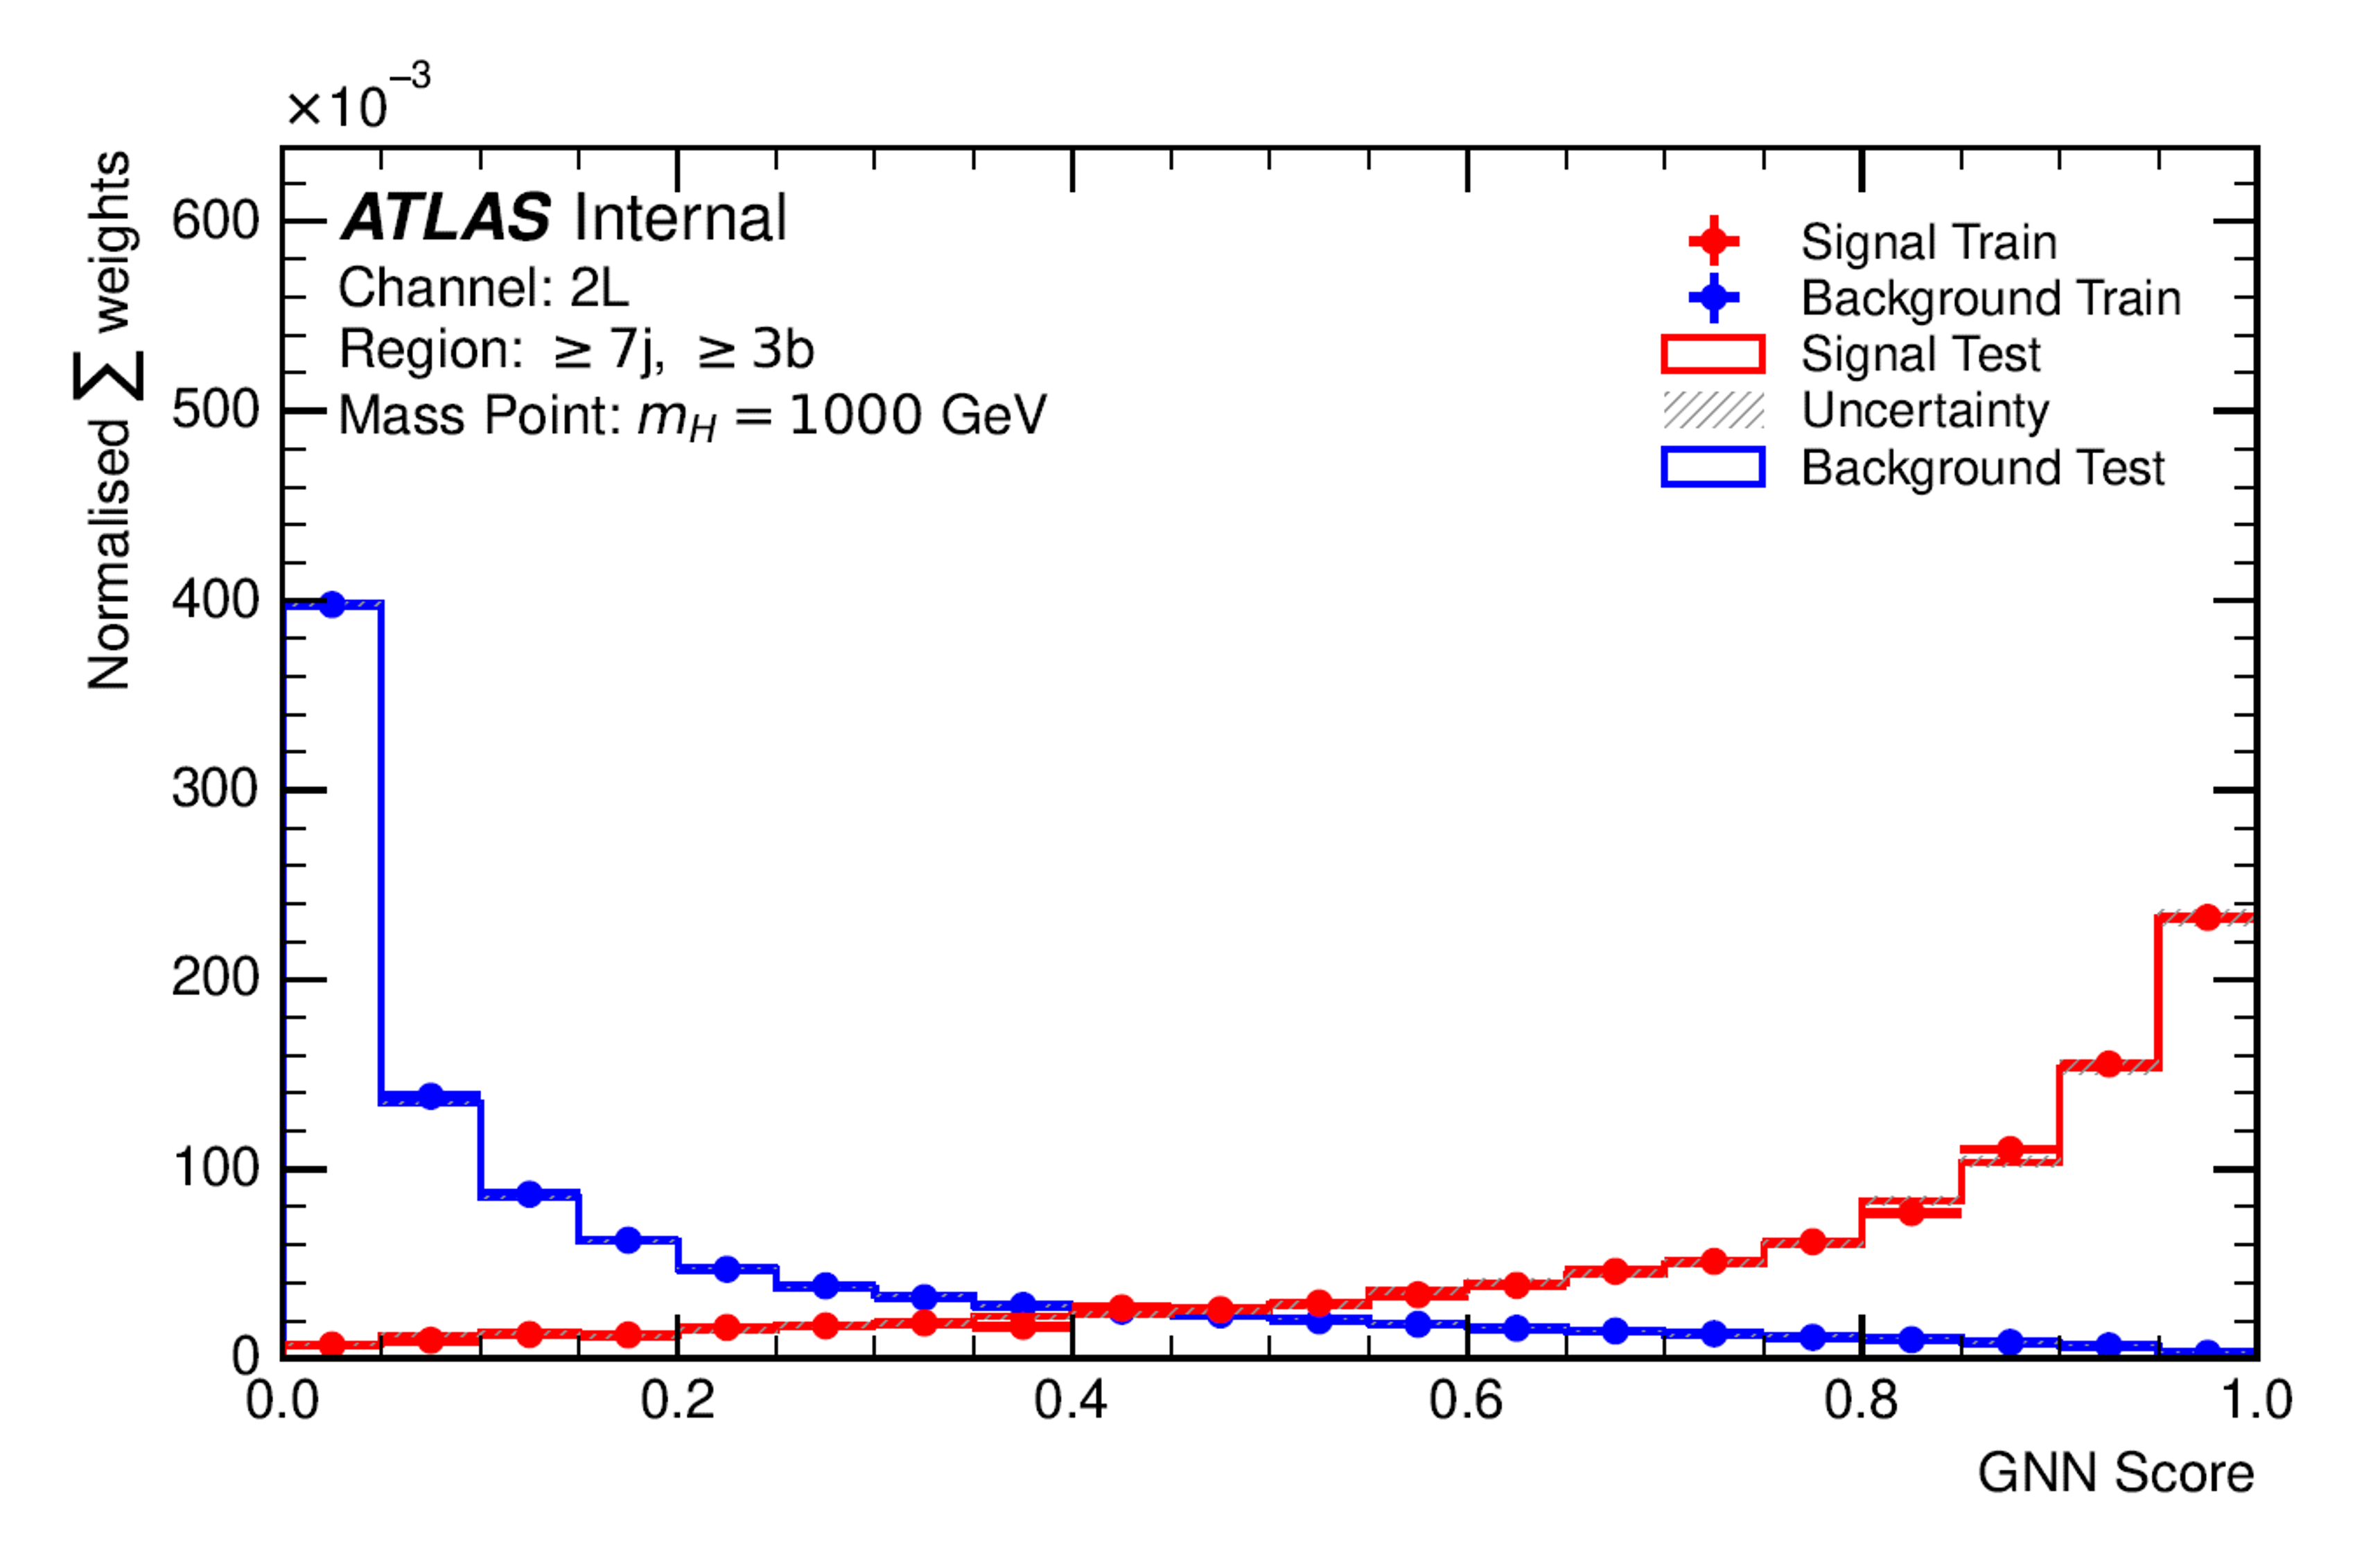
\includegraphics[width=\textwidth]{figures/gnn/Plots_2LOS/1000/GNN_Score_Plot_1000GeV_Inclusive.png}
    \caption{$m_H=1000~\mathrm{GeV}$}
  \end{subfigure}
  \caption{GNN score distributions in the 2LOS channel for representative Higgs-boson mass hypotheses in the inclusive training region.}
  \label{fig:2los-gnn-scores}
\end{figure}

The evolution of classifier performance as a function of the signal mass hypothesis is quantified using the AUC metric, as shown in Figure~\ref{fig:auc-vs-mass}. 
An increasing trend of AUC with increasing Higgs-boson mass is observed in both channels. 
This behaviour is consistent with the fact that heavier Higgs bosons lead to more energetic and more distinct event topologies, thereby enhancing the discriminating power of the multivariate classifier.

\begin{figure}[htbp]
  \centering
  \begin{subfigure}[t]{0.49\textwidth}
    \centering
    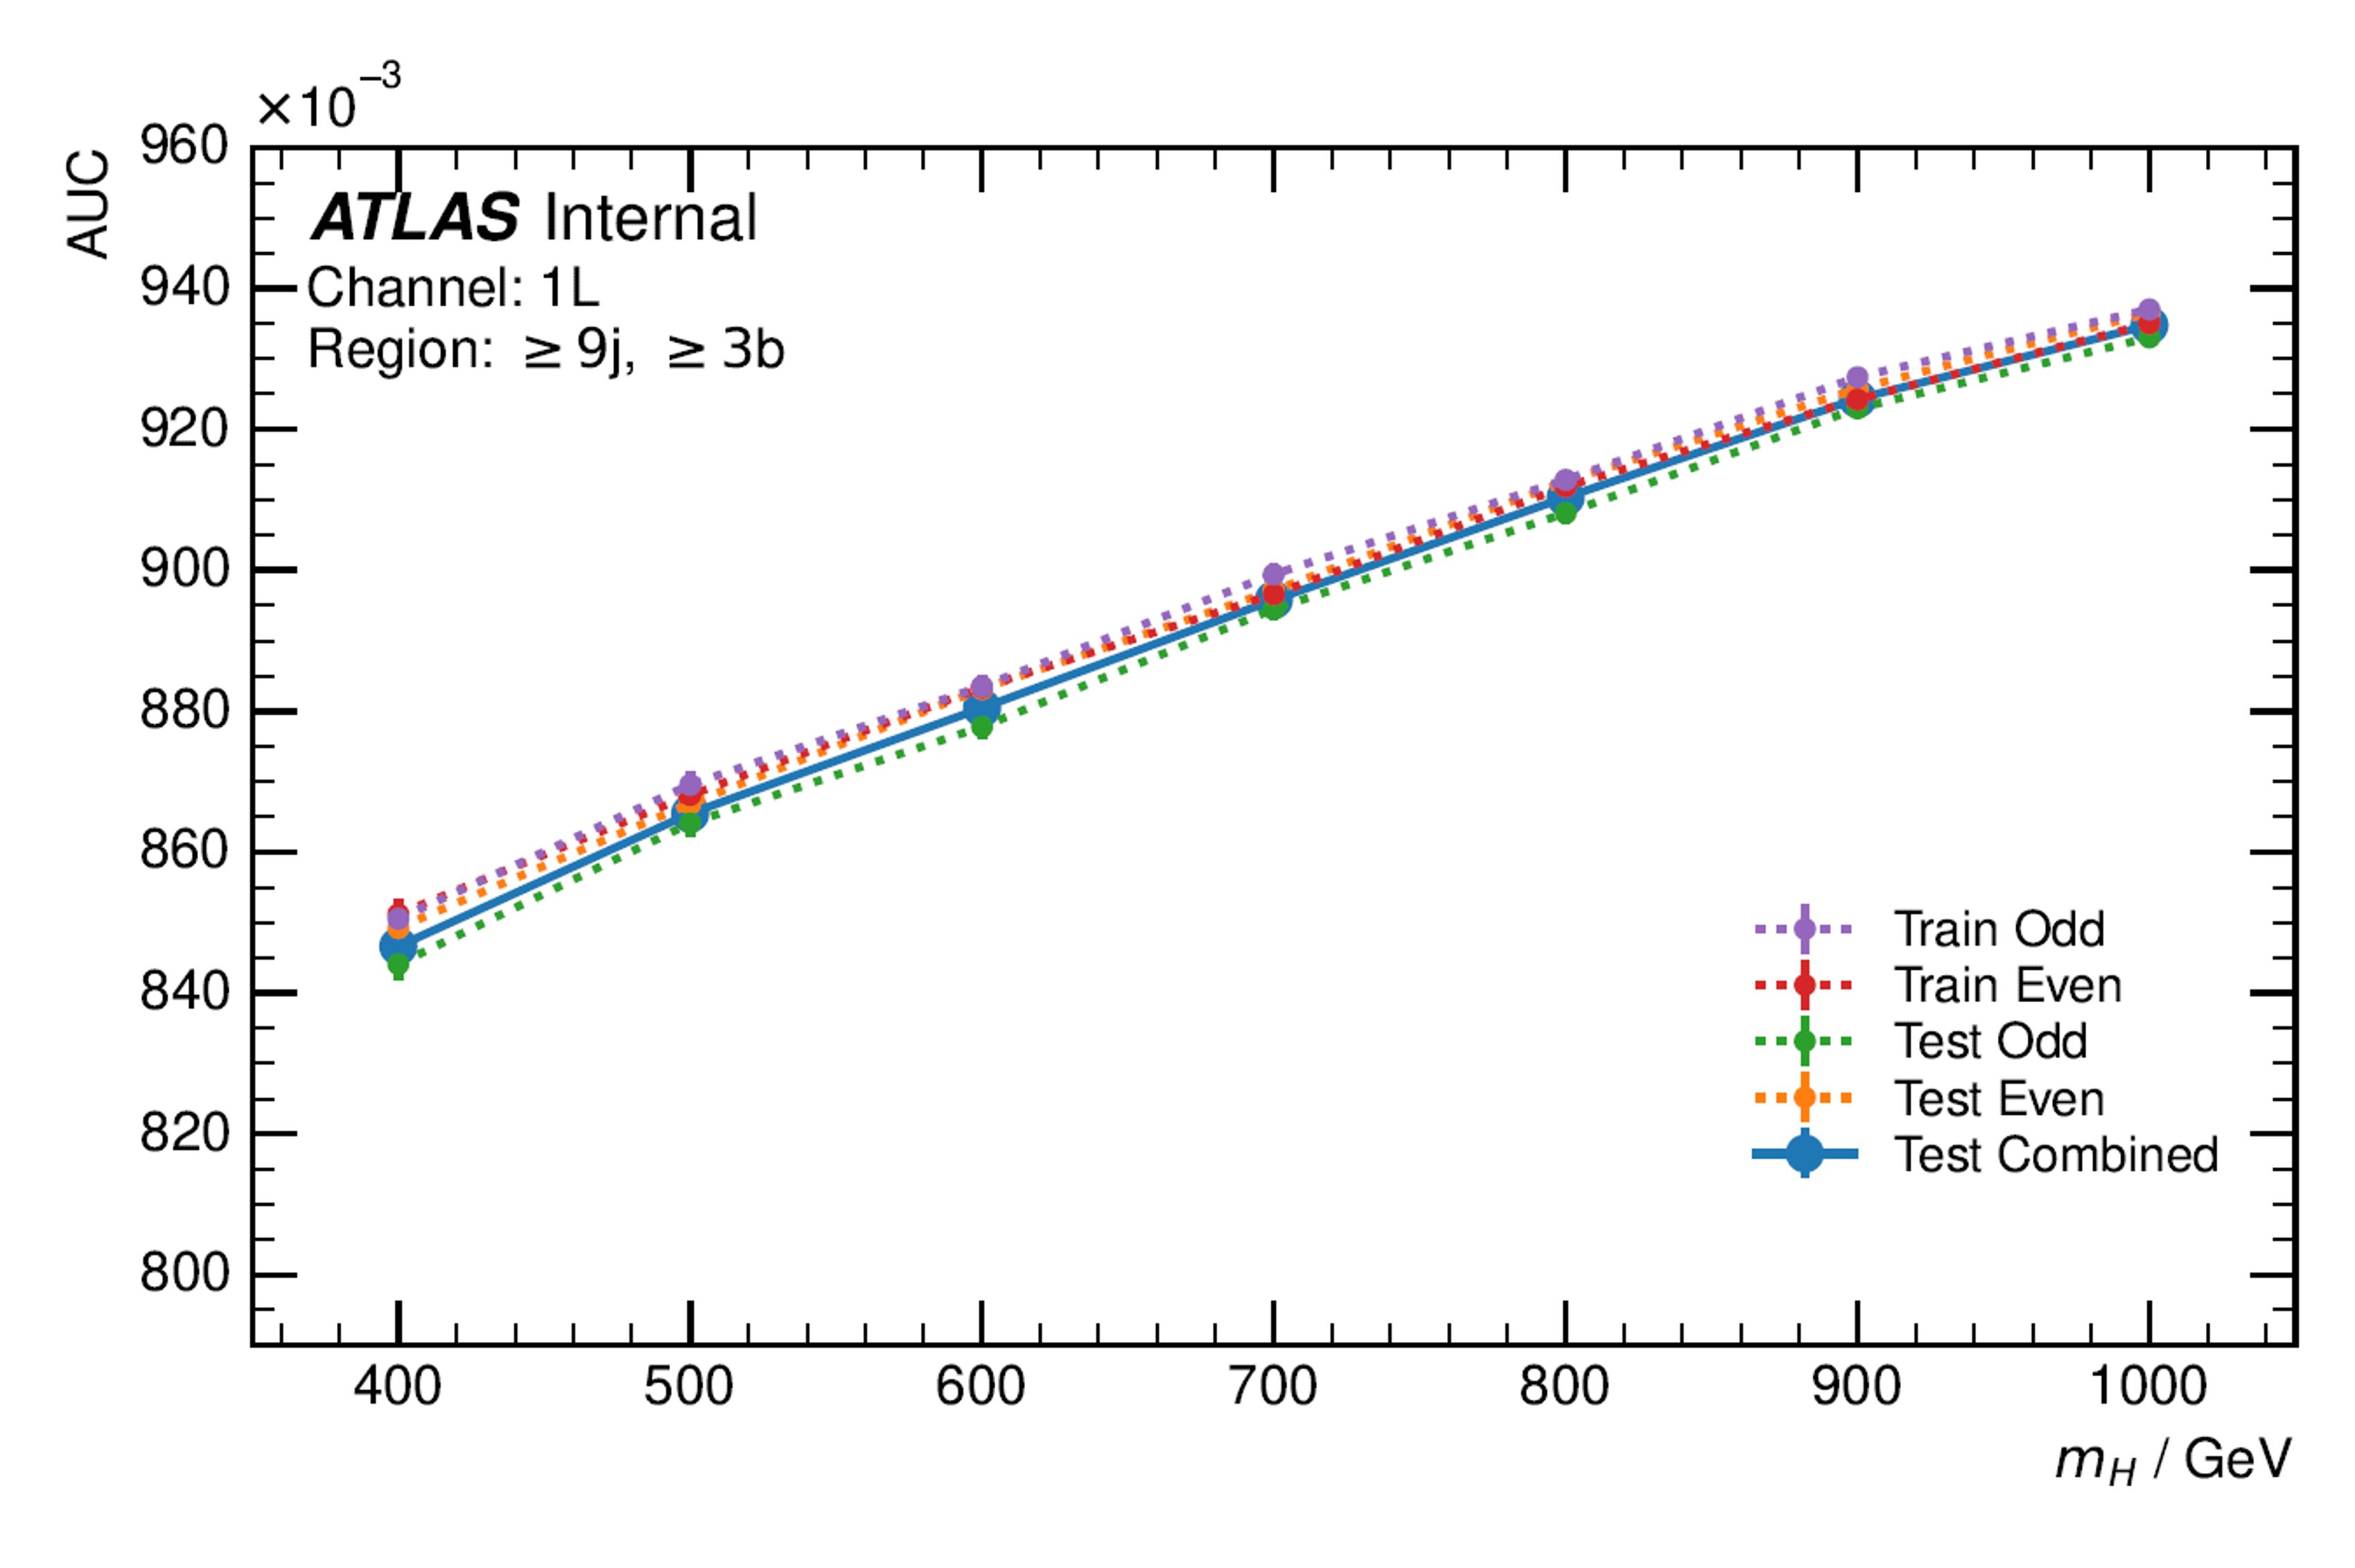
\includegraphics[width=\textwidth]{figures/gnn/Plots_1L/AUC_vs_Mass_Inclusive.png}
    \caption{1L channel}
  \end{subfigure}\hfill
  \begin{subfigure}[t]{0.49\textwidth}
    \centering
    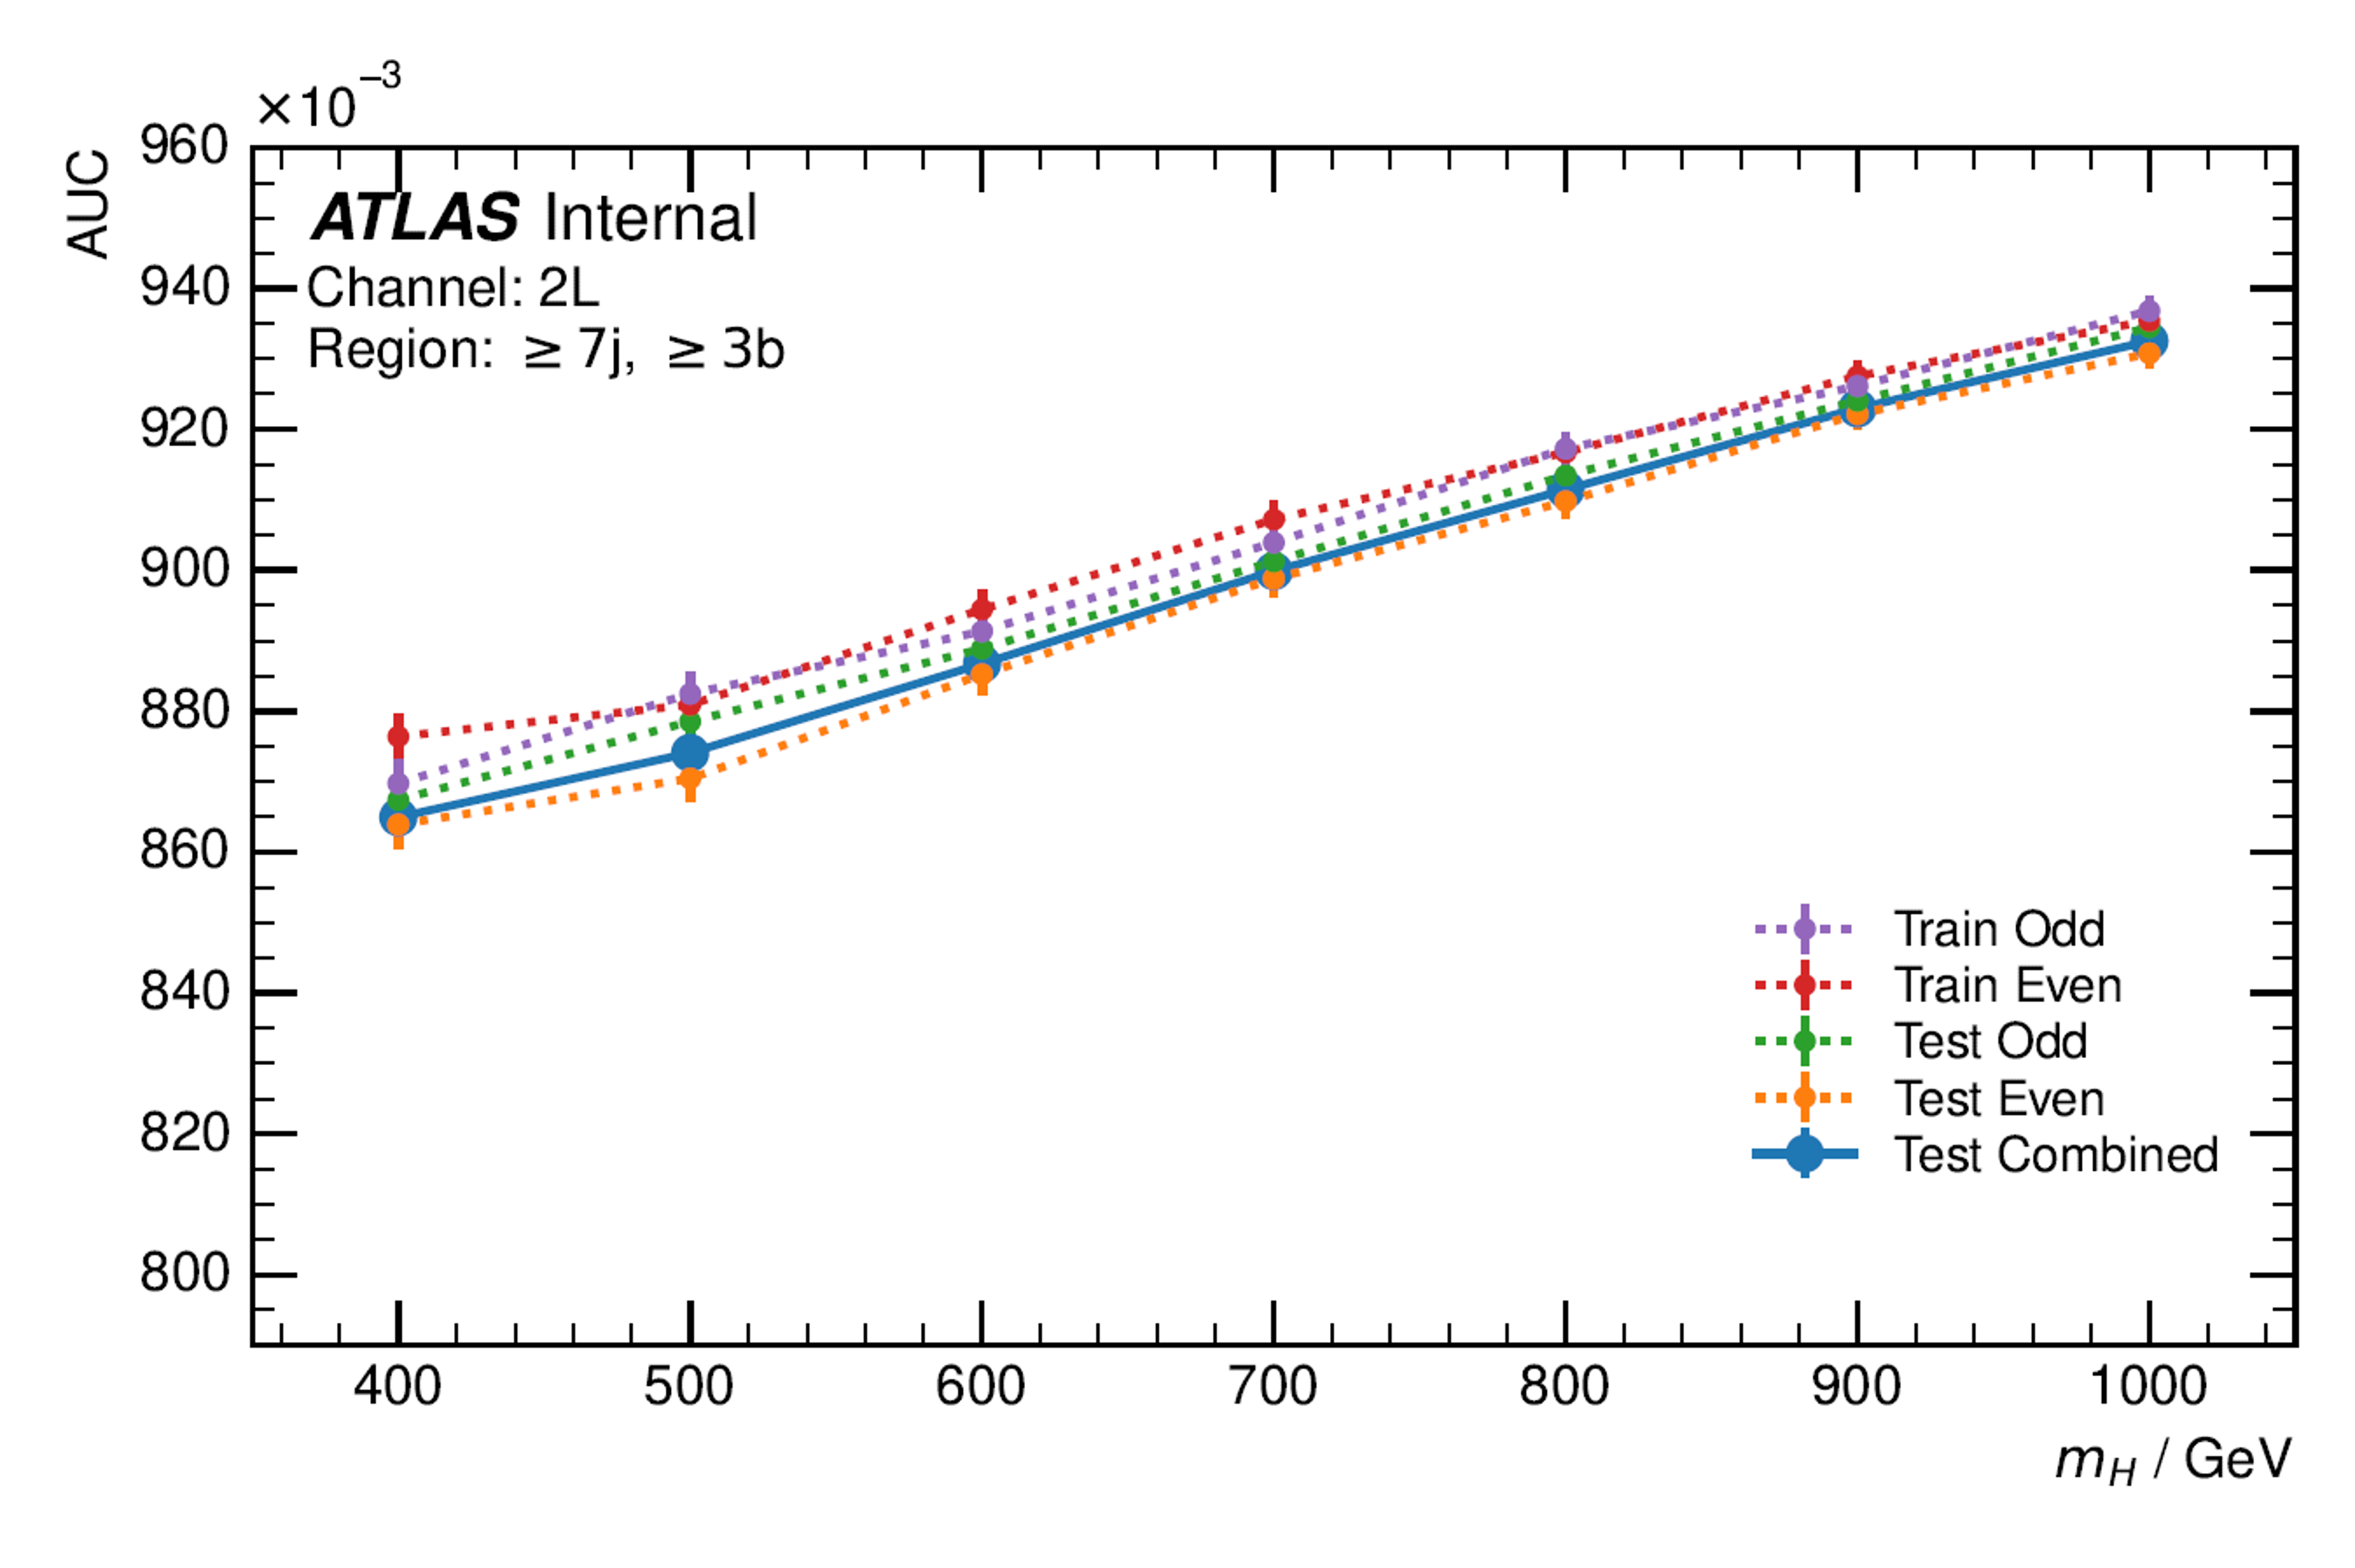
\includegraphics[width=\textwidth]{figures/gnn/Plots_2LOS/AUC_vs_Mass_Inclusive.png}
    \caption{2LOS channel}
  \end{subfigure}
  \caption{AUC as a function of the Higgs-boson mass hypothesis for the cross-trained GNN models.}
  \label{fig:auc-vs-mass}
\end{figure}

A dedicated study is performed to validate the mass-parameterised training strategy. 
For each simulated signal mass point, the classifier is evaluated using different mass hypotheses as input. 
The resulting AUC values are shown in Figure~\ref{fig:gnn-auc-matrix}. 
The performance is maximal when the evaluation mass hypothesis matches the true signal mass (diagonal entries), while deviations from the diagonal lead to reduced separation. 
This behaviour demonstrates that the network has learned a meaningful dependence on the mass parameter rather than treating it as a trivial input feature. 
It further confirms that the parameterised classifier effectively reproduces the behaviour of mass-specific classifiers within a unified framework.

\begin{figure}[htbp]
  \centering
  \begin{subfigure}[t]{0.49\textwidth}
    \centering
    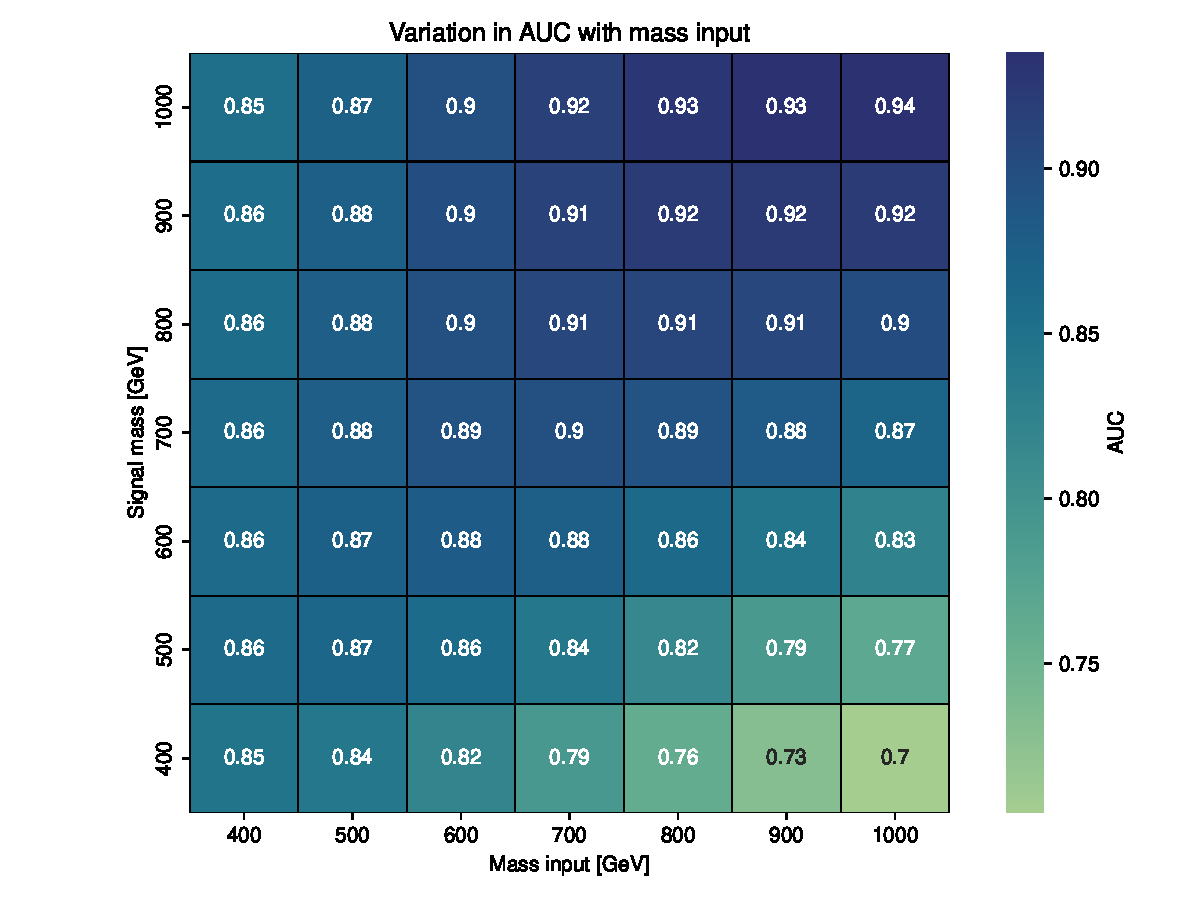
\includegraphics[width=\textwidth]{figures/gnn/Plots_1L/AUC_mass_variations.pdf}
    \caption{1L channel}
  \end{subfigure}\hfill
  \begin{subfigure}[t]{0.49\textwidth}
    \centering
    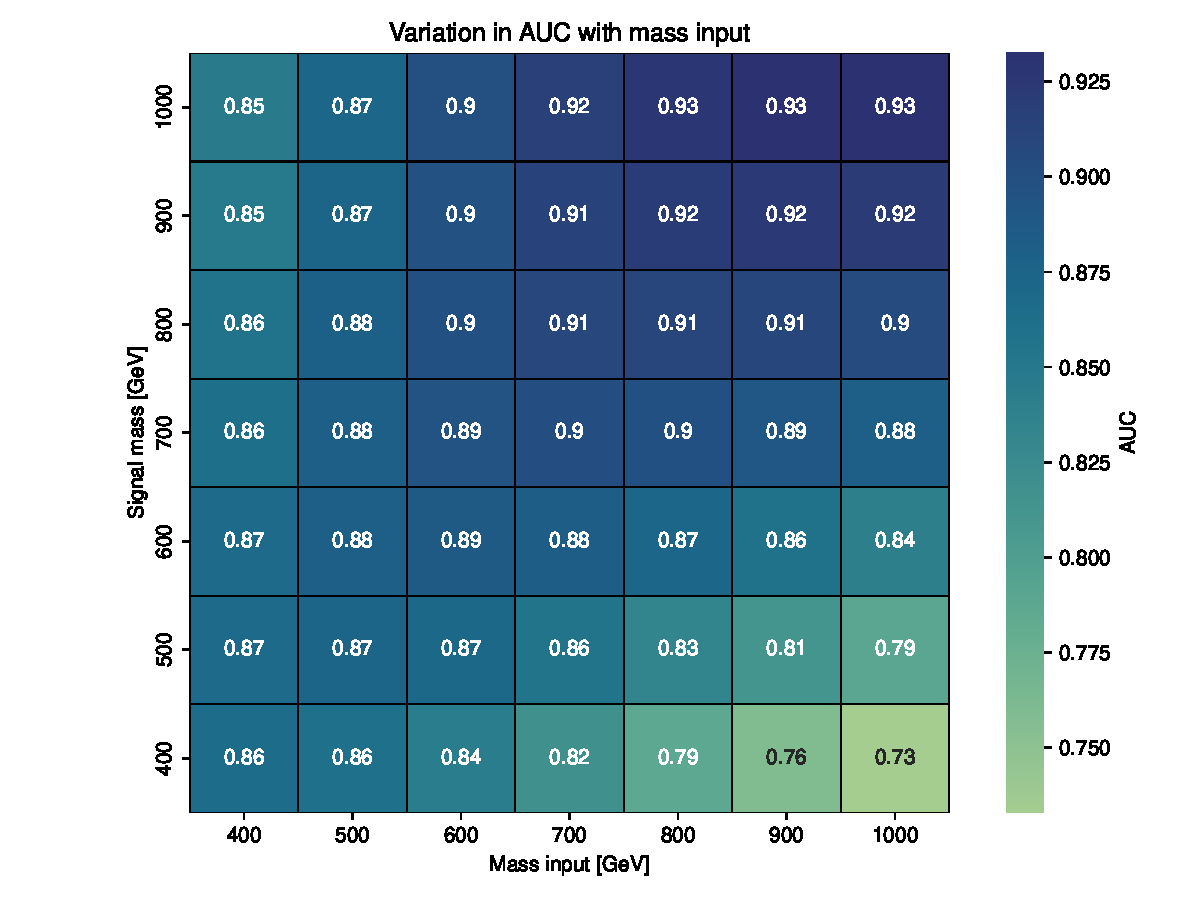
\includegraphics[width=\textwidth]{figures/gnn/Plots_2LOS/AUC_mass_variations.pdf}
    \caption{2LOS channel}
  \end{subfigure}
  \caption{AUC values evaluated for different combinations of true signal mass (vertical axis) and input mass hypothesis (horizontal axis).}
  \label{fig:gnn-auc-matrix}
\end{figure}

The relative importance of input features is evaluated using a permutation-based approach. 
For each feature, its values are randomly shuffled among events while keeping all other inputs fixed, and the resulting increase in the binary cross-entropy loss is measured:
\[
\Delta \mathcal{L}_i = \mathcal{L}_{\text{shuffled } i} - \mathcal{L}_{\text{nominal}}.
\]
Features that induce larger degradations in performance are considered more relevant for the classifier. 
The resulting ranking is shown in Figure~\ref{fig:gnn-feature-ranking}. 
High-level kinematic variables, $b$-tagging information, and relational features encoded in the graph are found to contribute significantly to the overall discrimination power. 
It should be noted that this method provides a global measure of feature relevance and may underestimate the importance of strongly correlated inputs.

\begin{figure}[htbp]
  \centering
  \begin{subfigure}[t]{0.49\textwidth}
    \centering
    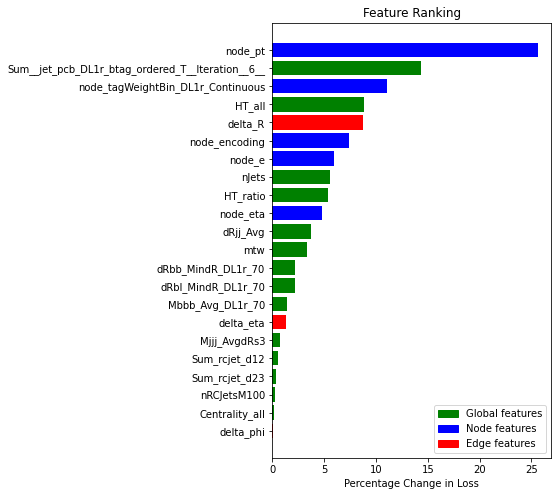
\includegraphics[width=\textwidth]{figures/gnn/Plots_1L/FeatureRanking_1L.png}
    \caption{1L channel}
  \end{subfigure}\hfill
  \begin{subfigure}[t]{0.49\textwidth}
    \centering
    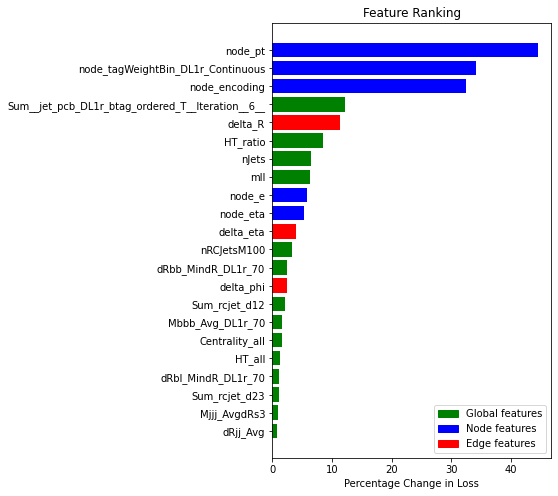
\includegraphics[width=\textwidth]{figures/gnn/Plots_2LOS/FeatureRanking_2LOS.png}
    \caption{2LOS channel}
  \end{subfigure}
  \caption{Permutation-based feature importance ranking for the mass-parameterised GNN classifier.}
  \label{fig:gnn-feature-ranking}
\end{figure}

Overall, the validation studies demonstrate that the mass-parameterised GNN classifier provides stable and robust discrimination across all benchmark mass points. 
The classifier is therefore used as the nominal discriminant in the subsequent statistical interpretation.
